%
% test_report_v05.tex
%
% Copyright (C) 2021 by SpaceLab.
%
% EPS 2.0 Documentation
%
% This work is licensed under the Creative Commons Attribution-ShareAlike 4.0
% International License. To view a copy of this license,
% visit http://creativecommons.org/licenses/by-sa/4.0/.
%

%
% \brief Test report of the v0.1 hardware.
%
% \author André M. P. Mattos <andre.mattos@spacelab.ufsc.com>
%
% \institution Universidade Federal de Santa Catarina (UFSC)
%
% \version 0.1.0
%
% \date 2021/06/23
%

\chapter{Test Report of v0.2 Version} \label{anx:test-report-v02}

This appendix is a test report of the first manufactured and assembled PCB (version v0.2).

\begin{itemize}
    \item \textbf{PCB manufacturer}: PCBWay (China)
    \item \textbf{PCB assembly}: PCBWay (China)
    \item \textbf{PCB arrival date}: 2022/04/14 
    \item \textbf{Execution date}: 2022/04/15 to 2022/05/15
    \item \textbf{Tester}: João Cláudio and Ramon Borba
\end{itemize}

\section{Visual Inspection}

\begin{figure}[!ht]
    \begin{center}
        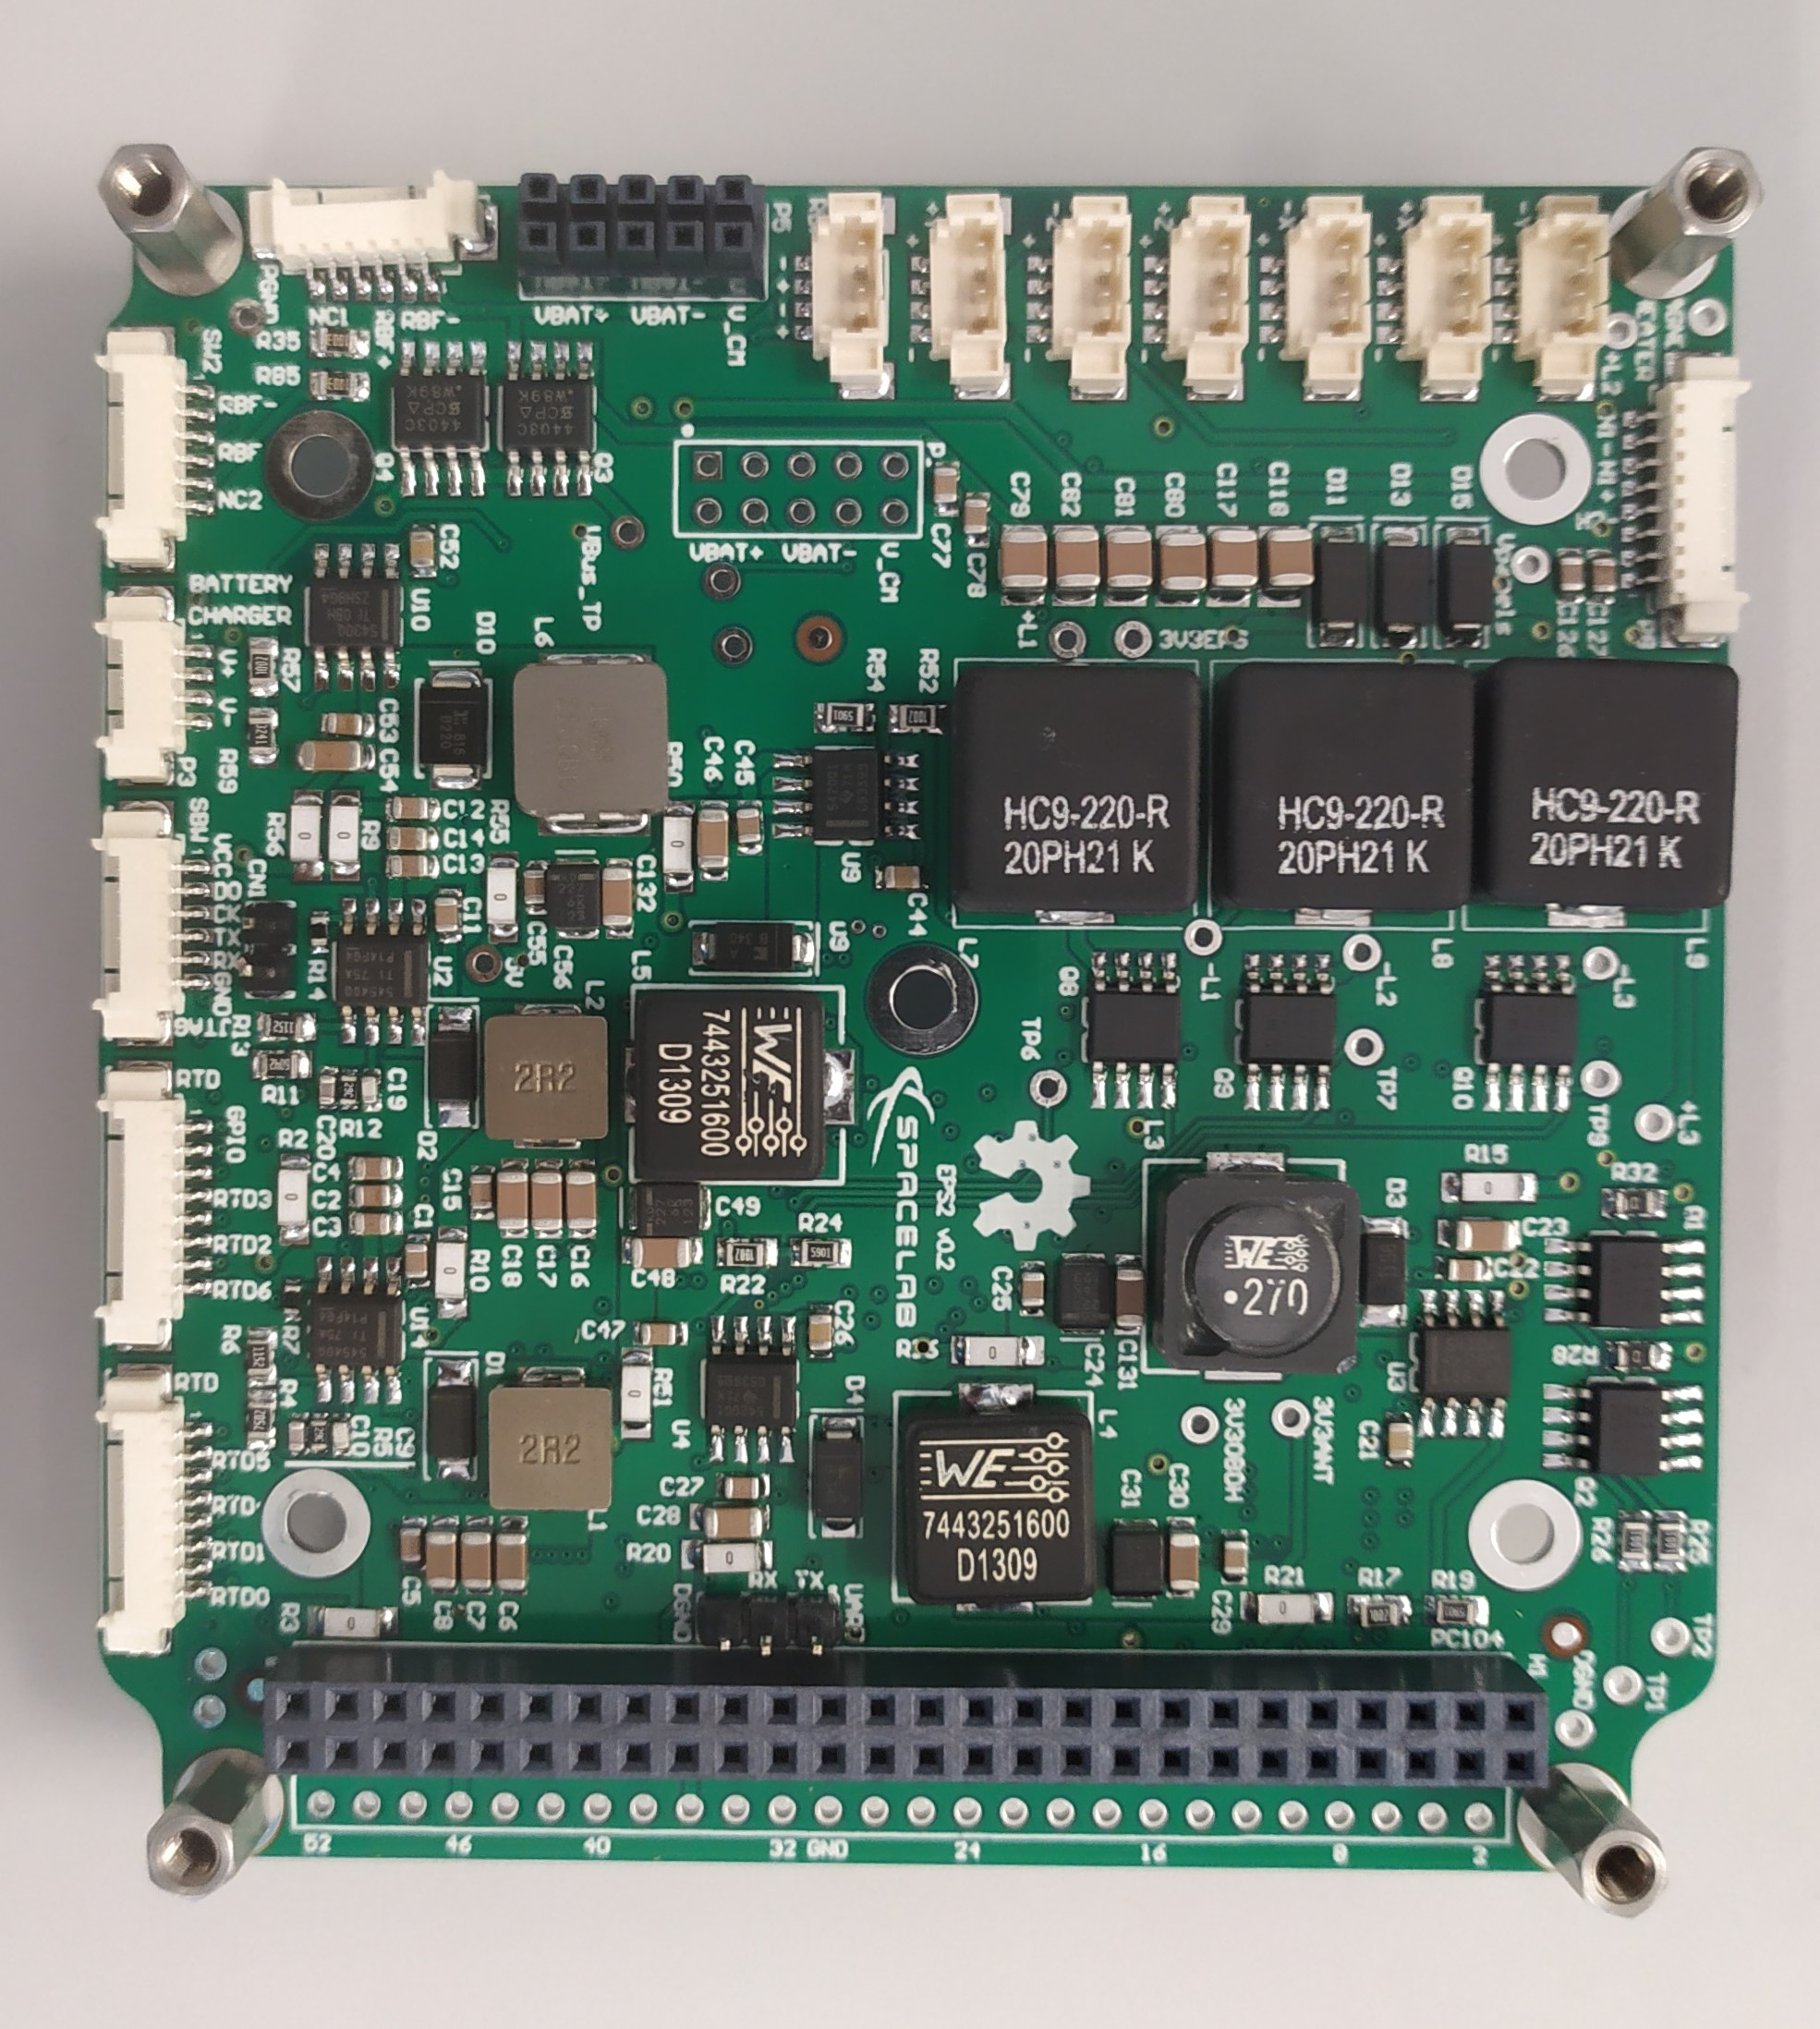
\includegraphics[width=0.6\columnwidth]{figures/v02/eps2-v02-top.jpg}
        \caption{Top view of the EPS 2.0 v0.2 board.}
        \label{fig:eps2-v01-top}
    \end{center}
\end{figure}

\begin{figure}[!ht]
    \begin{center}
        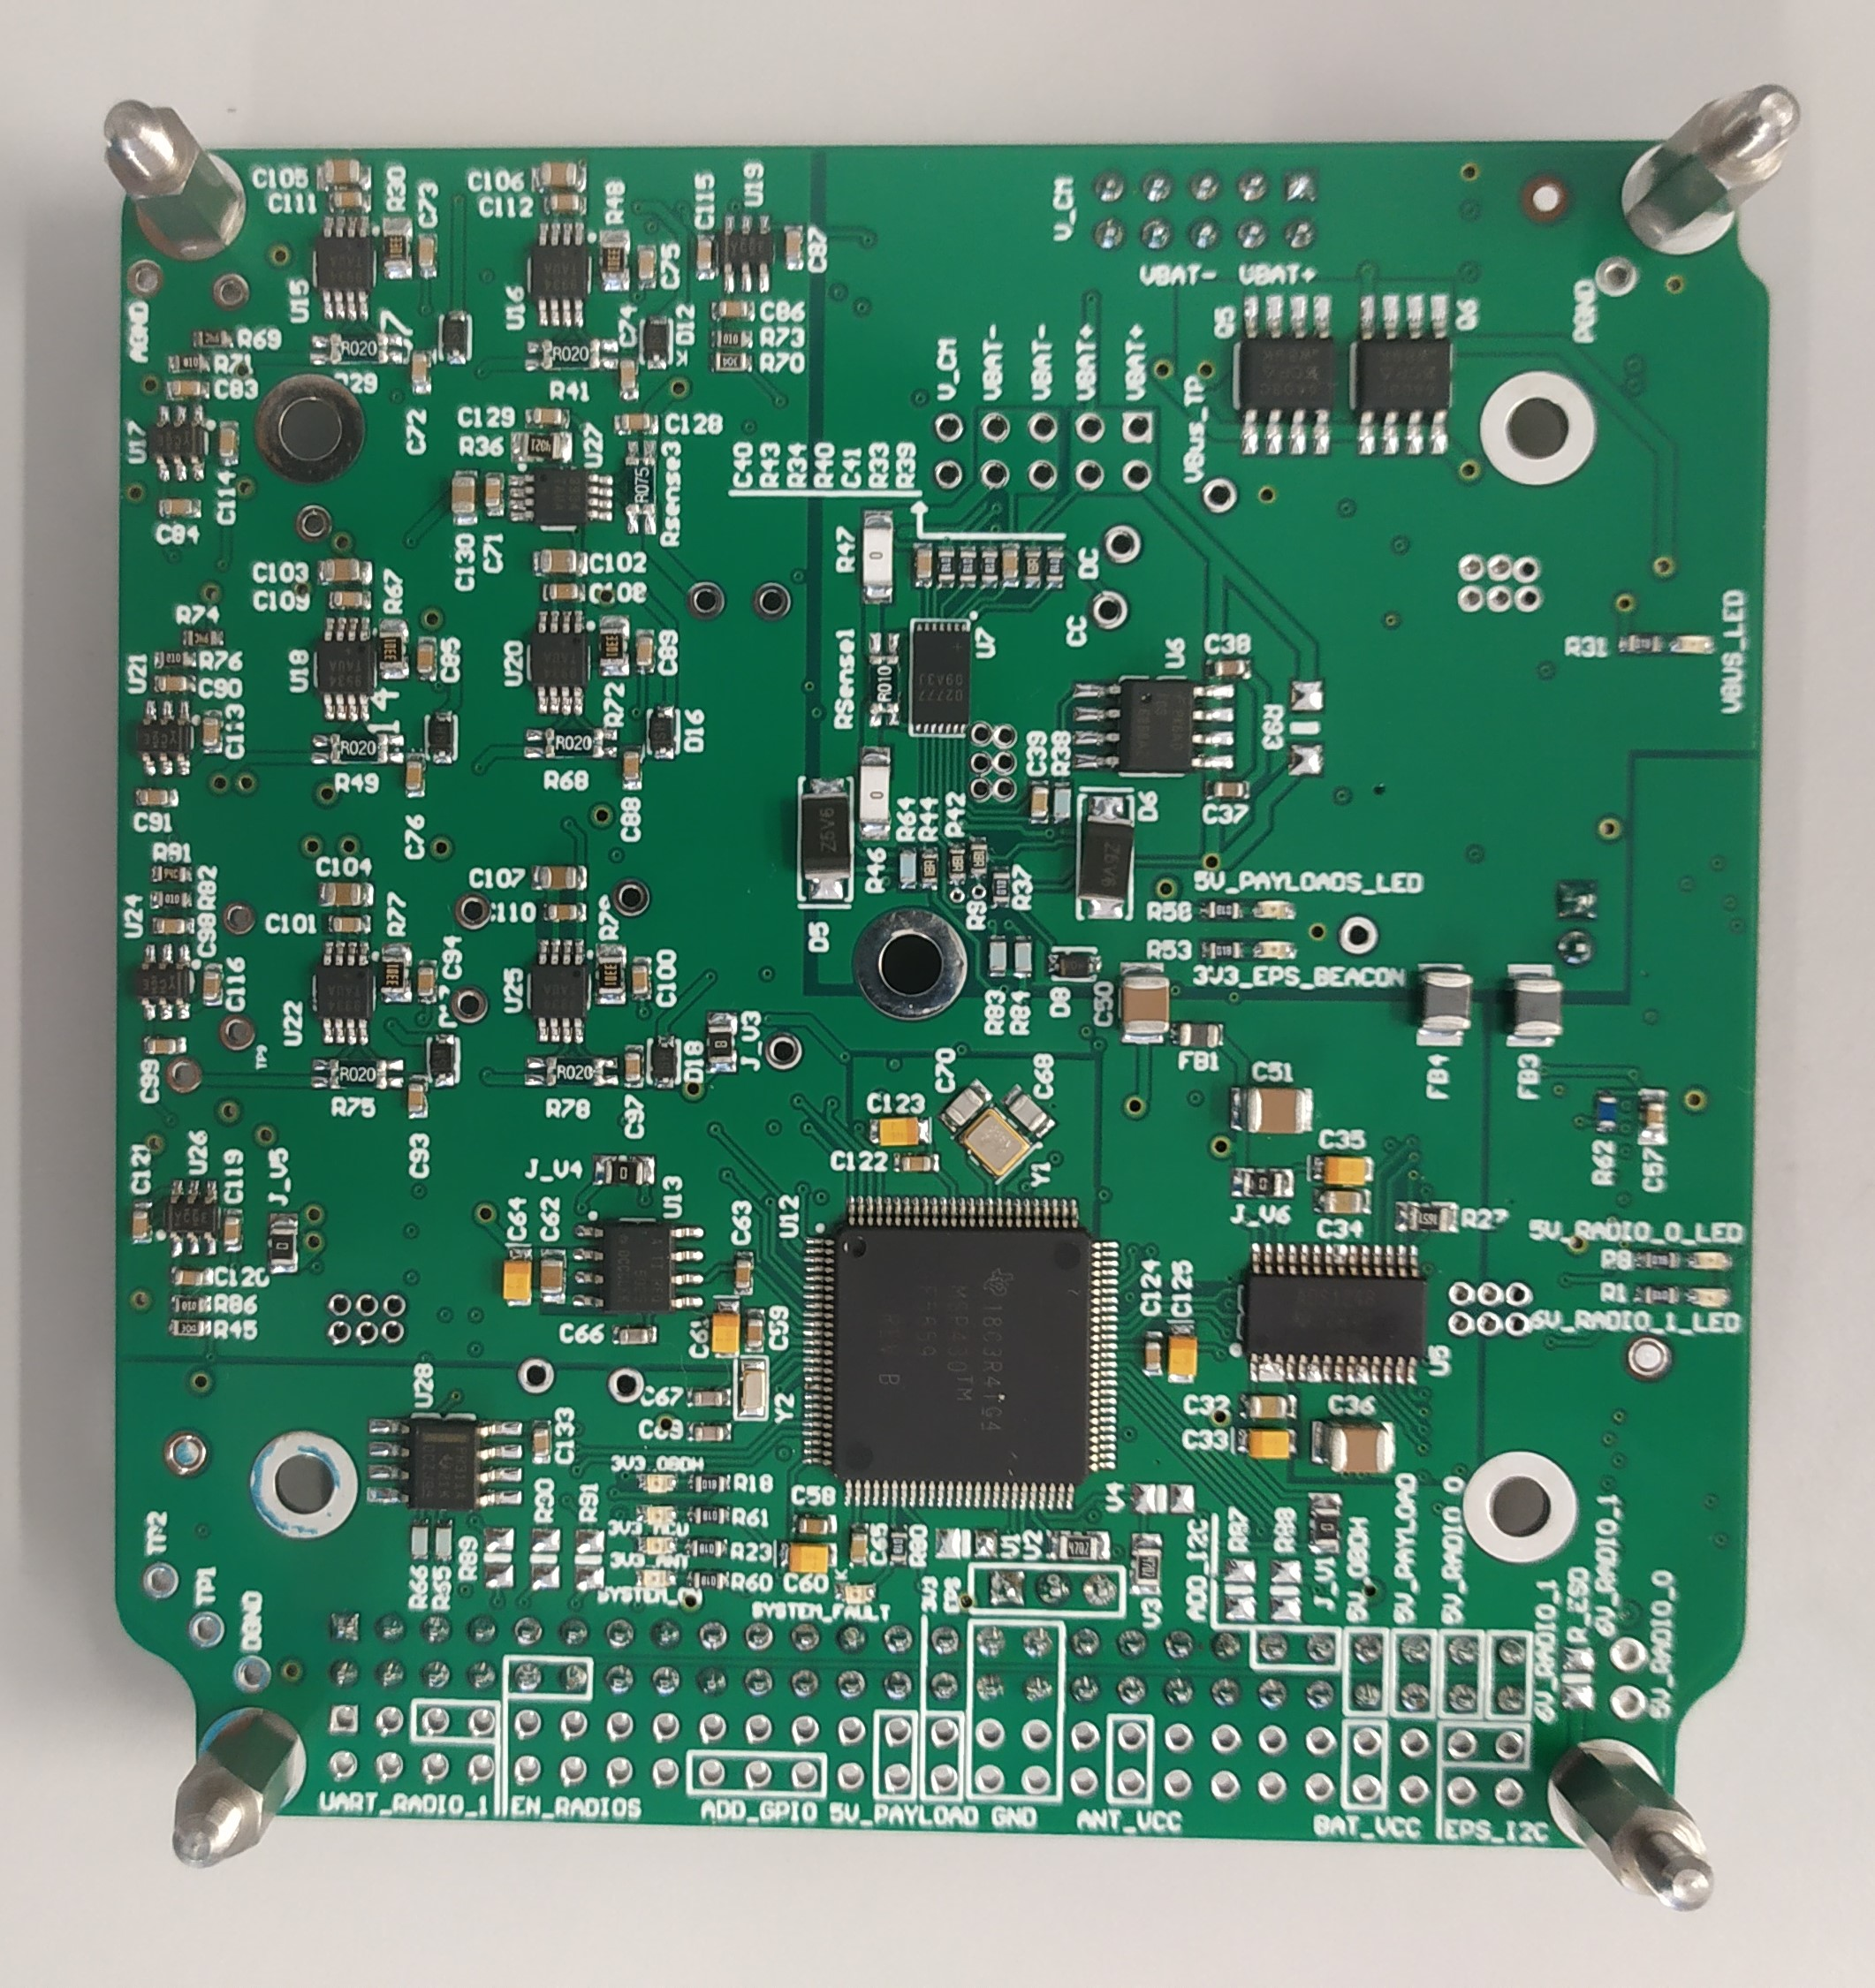
\includegraphics[width=0.6\columnwidth]{figures/v02/eps2-v02-bottom.jpg}
        \caption{Bottom view of the EPS 2.0 v0.2 board.}
        \label{fig:eps2-v01-bottom}
    \end{center}
\end{figure}

\begin{itemize}
    \item \textbf{Test description/Objective}: Inspection of the board, visually, searching for fabrication and assembly failures.
    \item \textbf{Procedures:} \autoref{tab:visual-inspection}.
    \item \textbf{Material}: None.
    \item \textbf{Results}: First, the top and bottom side of the EPS 2.0 are shown in \autoref{fig:eps2-v01-top} (top view of the board) and \autoref{fig:eps2-v01-bottom} (bottom view of the board). It was possible to see that some components were not soldered. At the bottom side the R89, R90, R91, versioning resistors V1 and V4, R93, R87, R88, R\_ESD were not soldered. At the top side only half of the PC-104 and P1 were not connected. Furthermore, the P5 was connected in the wrong side.
    \item \textbf{Conclusion}: No major problems were identified on this test.  
\end{itemize}

\newpage

\section{Mechanical Inspection}

\begin{itemize}
    \item \textbf{Test description/Objective}: Evaluate if the board has the right dimensions and the necessary mechanical specs prior to integration.
    \item \textbf{Procedures:} \autoref{tab:mechanical-inspection}.
    \item \textbf{Material}: Pachymeter, rule and a digital scale.
    \item \textbf{Results}: The inspection was performed with the available tools. The board presented the right dimensions and has 90g.
    \item \textbf{Conclusion}: The board should not present any problem due to the heritage from the previous models and the good manufacturing quality.
\end{itemize}


\section{Integration Inspection}

\begin{itemize}
    \item \textbf{Test description/Objective}: Analyze the integration accordance prior to the module’s full assembly on the CubeSat.
    \item \textbf{Procedures:} \autoref{tab:integration-inspection}.
    \item \textbf{Material}: None.
    \item \textbf{Results}: Schematic files and pinout identified in the \autoref{ch:hardware}. 
    \item \textbf{Conclusion}: No problems were identified on this test, except from those found during the visual inspection.
\end{itemize}


\section{Electrical Inspection}

\begin{itemize}
    \item \textbf{Test description/Objective}: Inspect for visually detectable electrical errors.
    \item \textbf{Procedures:} \autoref{tab:electrical-inspection}.
    \item \textbf{Material}: None.
    \item \textbf{Results}: The top and bottom side of the EPS 2.0 are shown in \autoref{fig:eps2-v01-top} (top view of the board) and \autoref{fig:eps2-v01-bottom} (bottom view of the board).
    \item \textbf{Conclusion}: No problems were identified on this test, components were correctly selected, placed and soldered (except for those already mentioned in the visual inspection).
\end{itemize}

\newpage

\section{Electrical Testing}

\begin{figure}[!htb]
    \begin{center}
        \subfigure[5V bus to the payload.\label{fig:5v_payload_bus}]{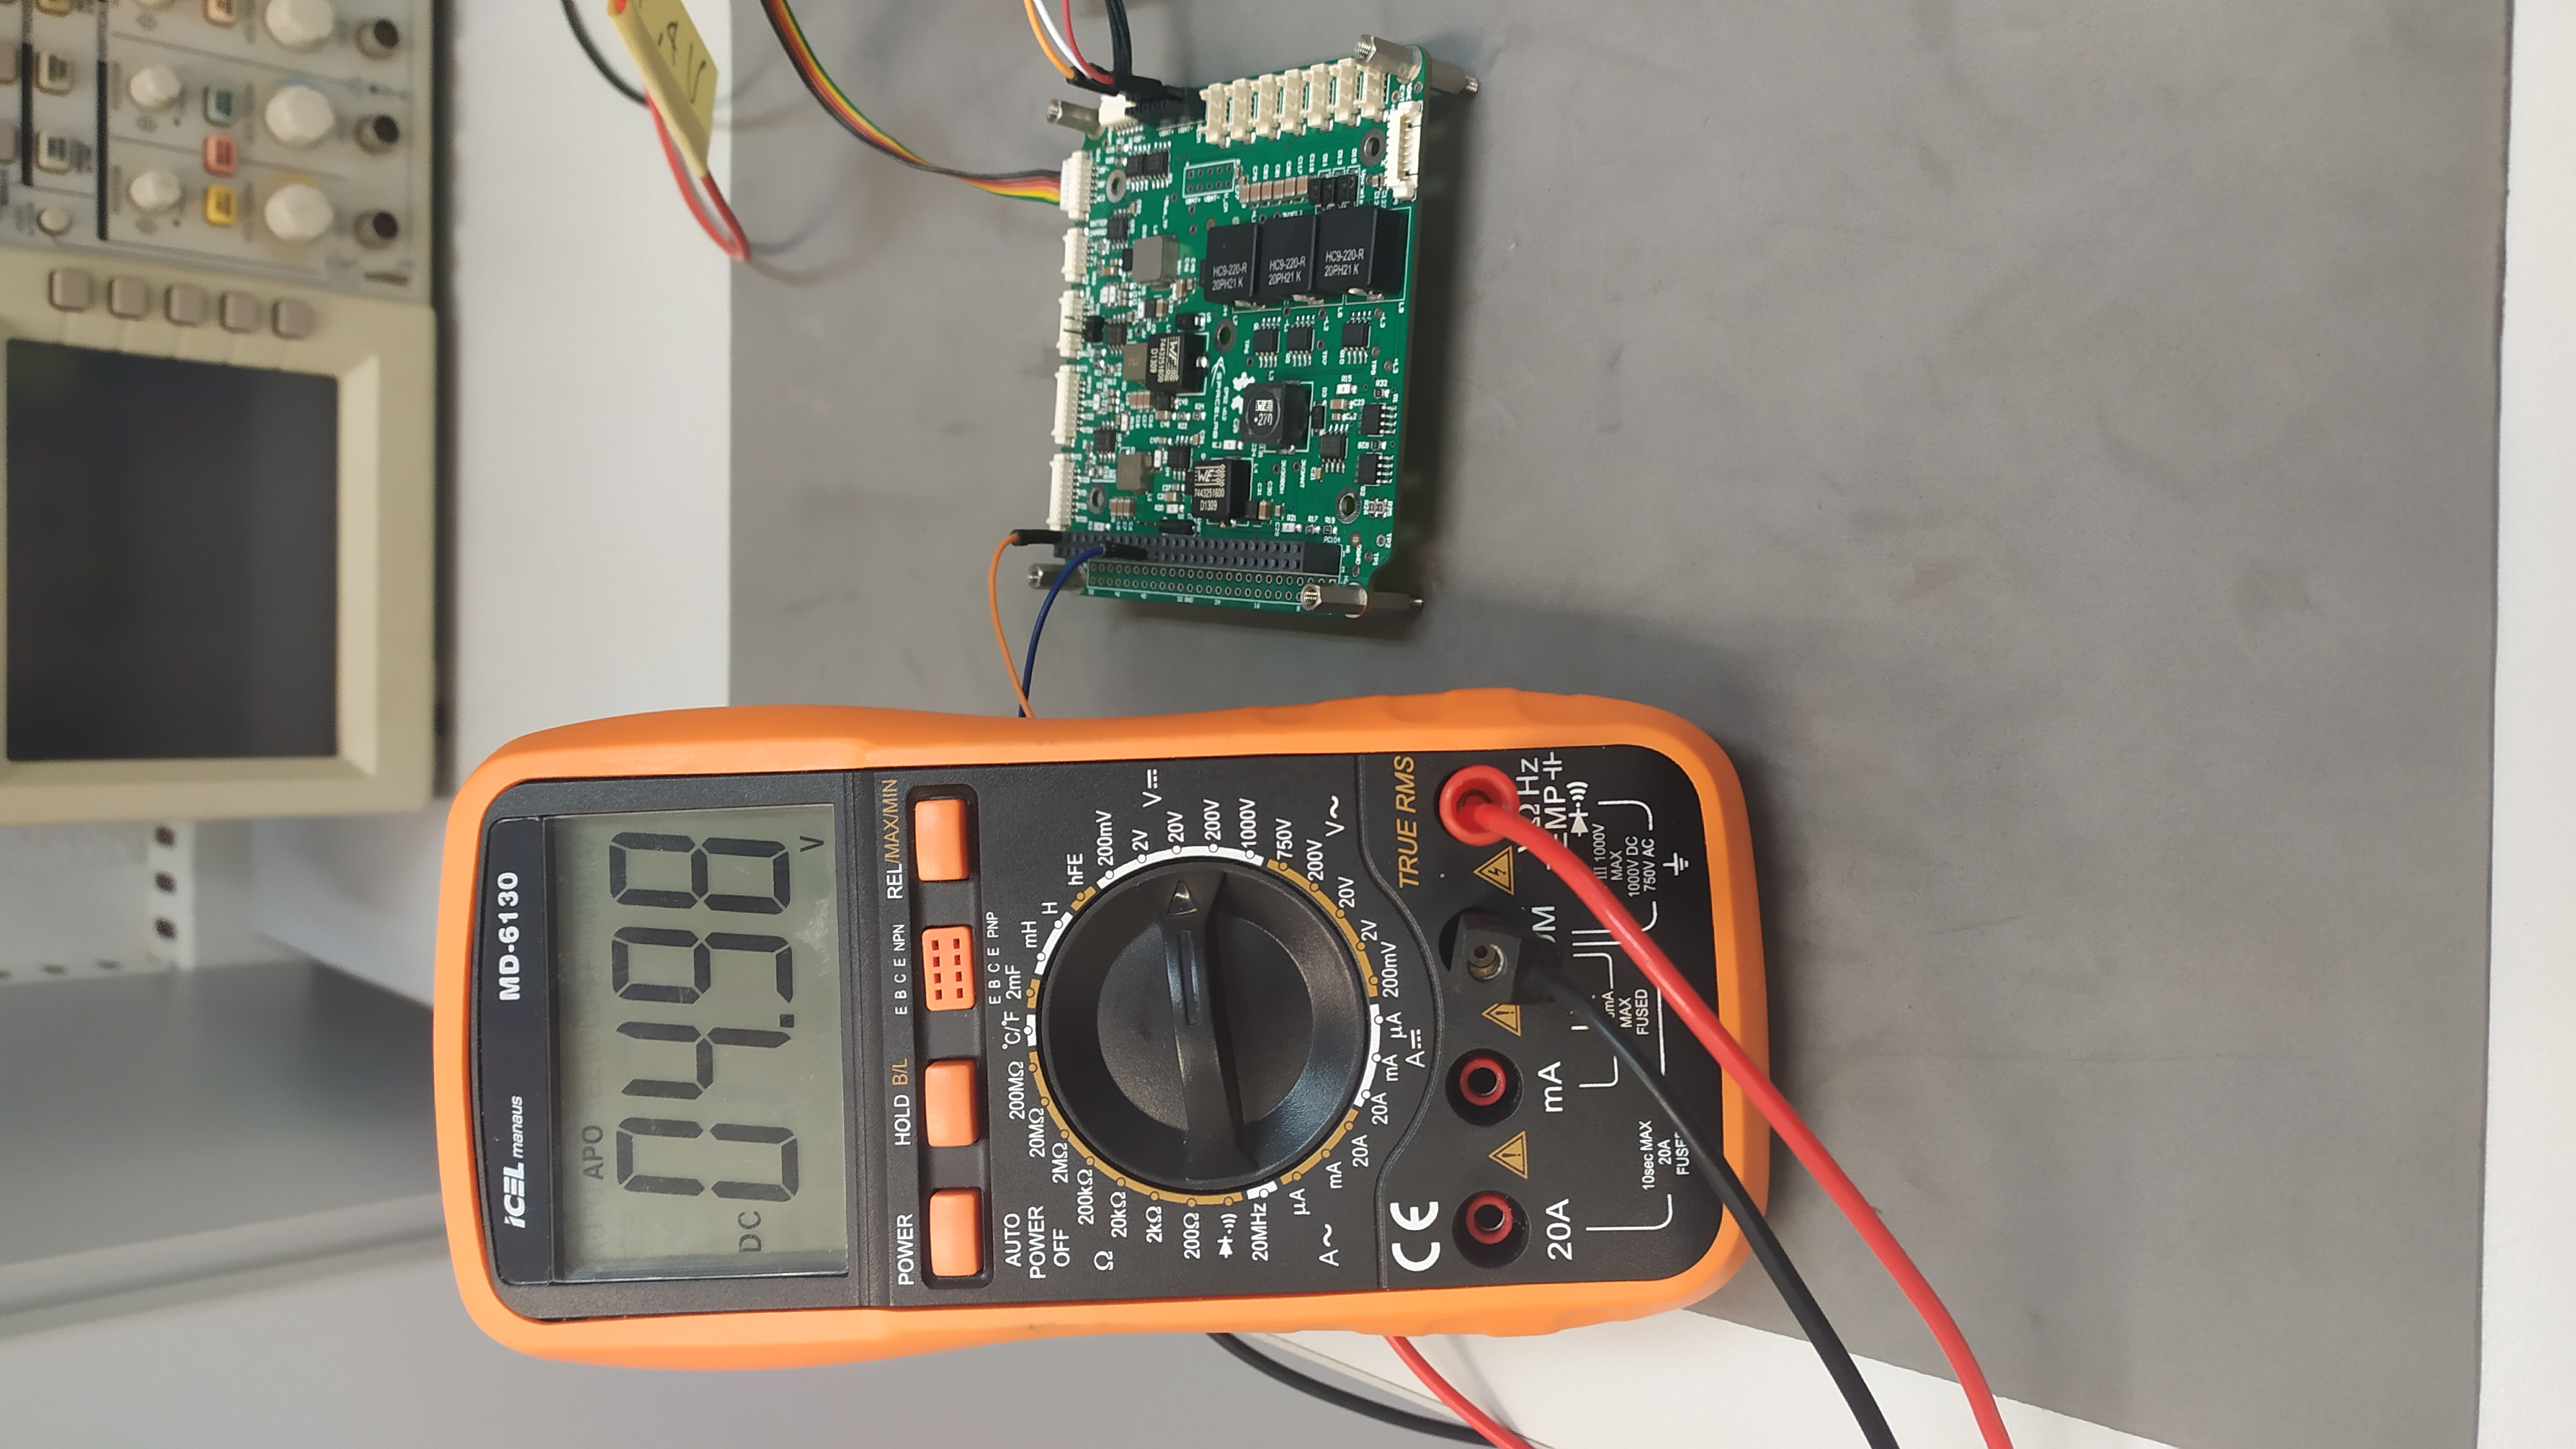
\includegraphics[angle=270,width=0.35\linewidth]{figures/v02/5v_payload_bus.jpg}}
        \hspace{10pt}%
        \subfigure[5V bus to the TTC.\label{fig:5v_radio_0_bus}]{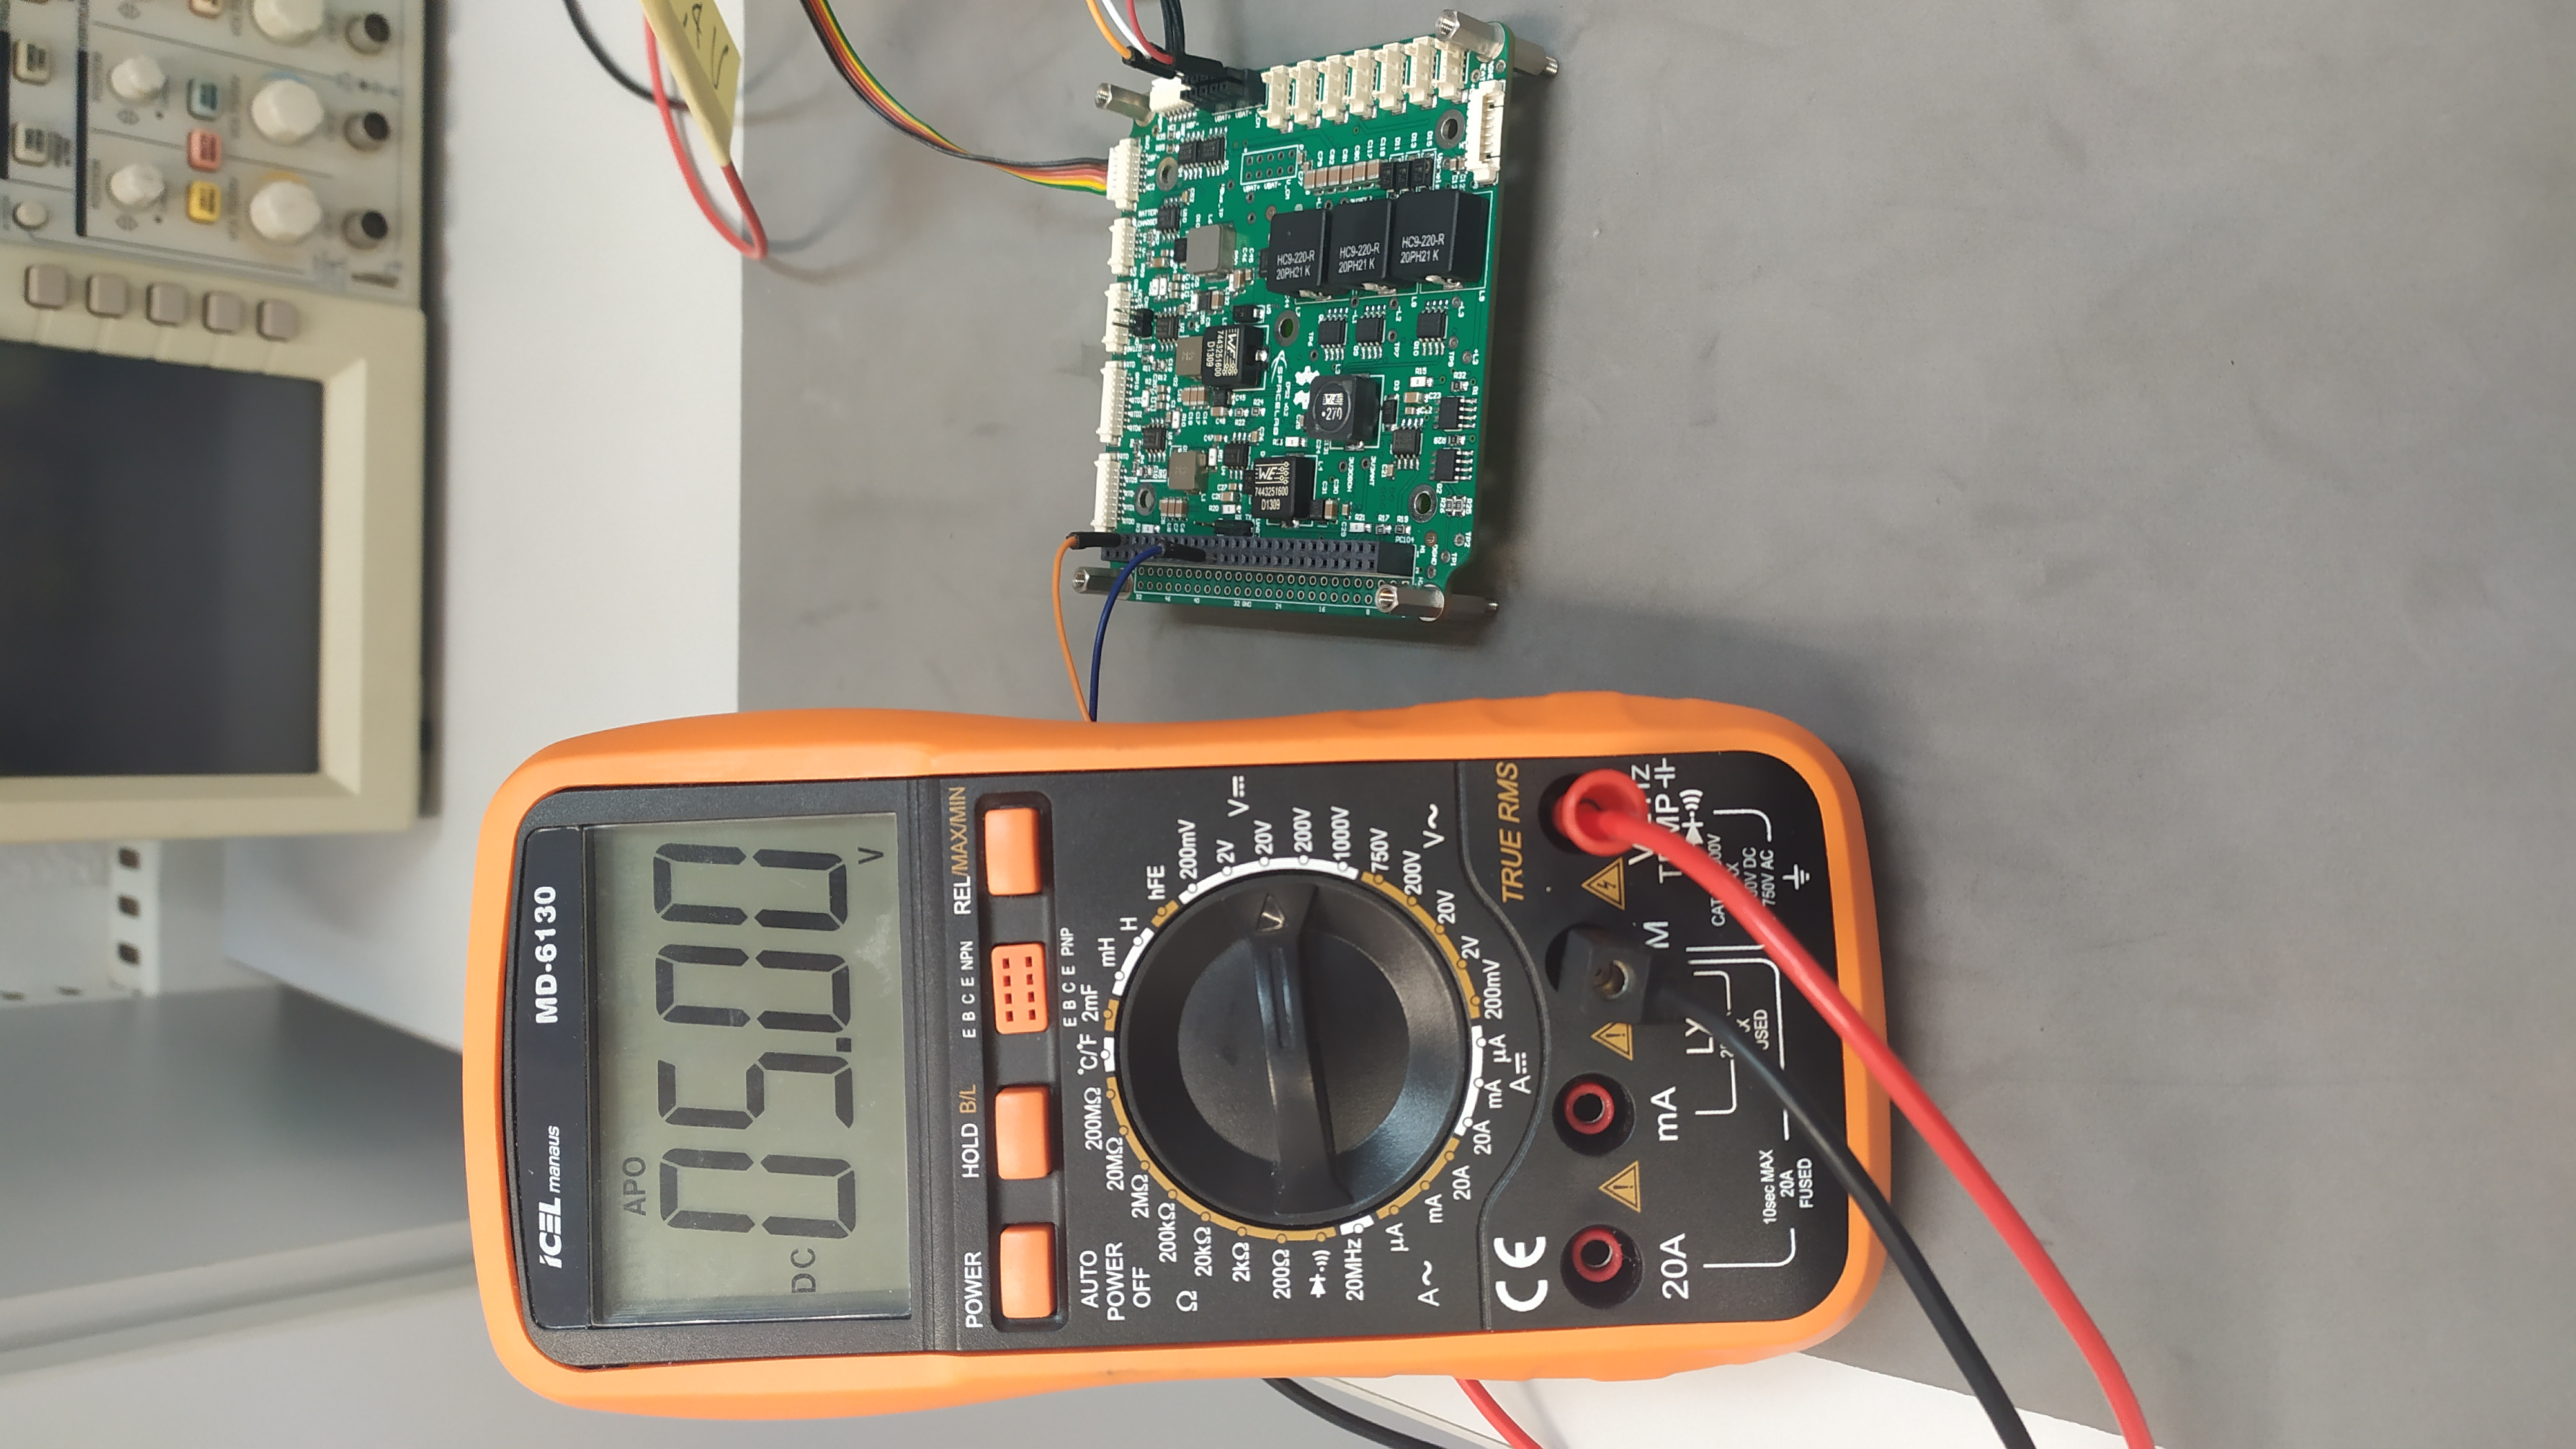
\includegraphics[angle=270,width=0.35\linewidth]{figures/v02/5v_radio_0_bus.jpg}} \\
        
        \subfigure[6V bus to the TTC.\label{fig:6v_radio_1_bus}]{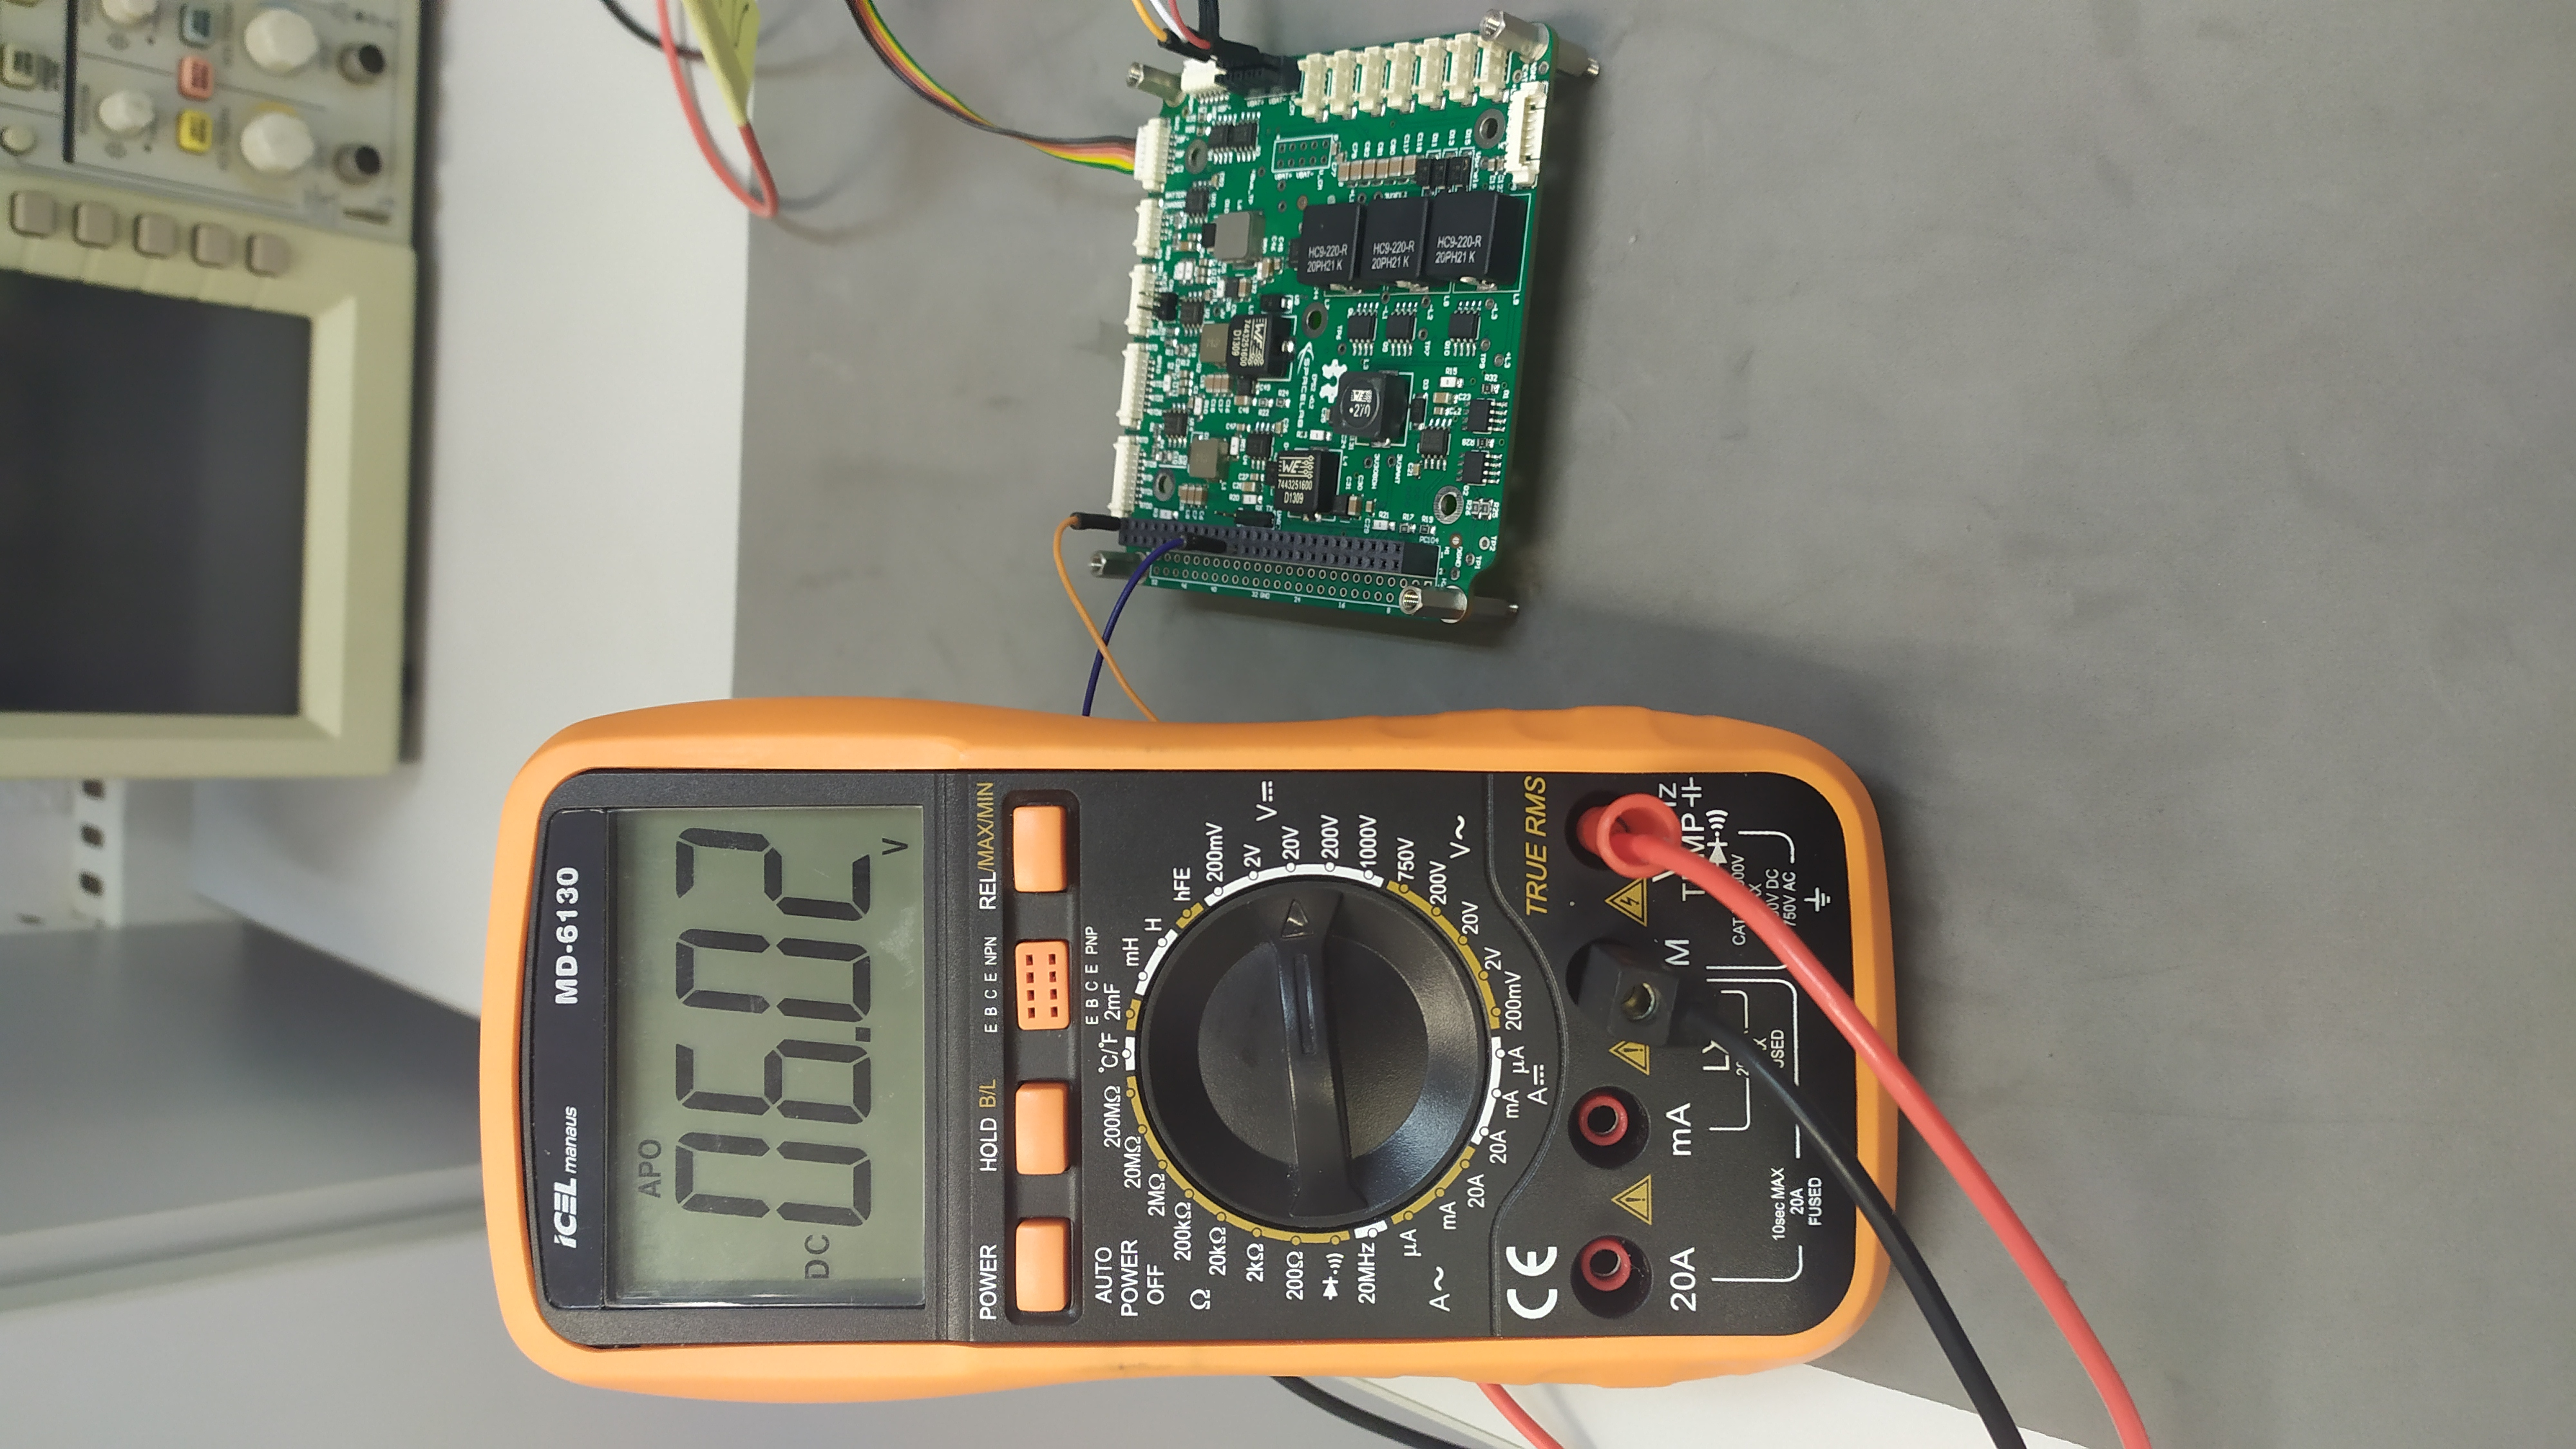
\includegraphics[angle=270,width=0.35\linewidth]{figures/v02/6v_radio_1_bus.jpg}}
        \hspace{10pt}%
        \subfigure[3,3V bus to multiple modules.\label{fig:3v3_all_modules_buses}]{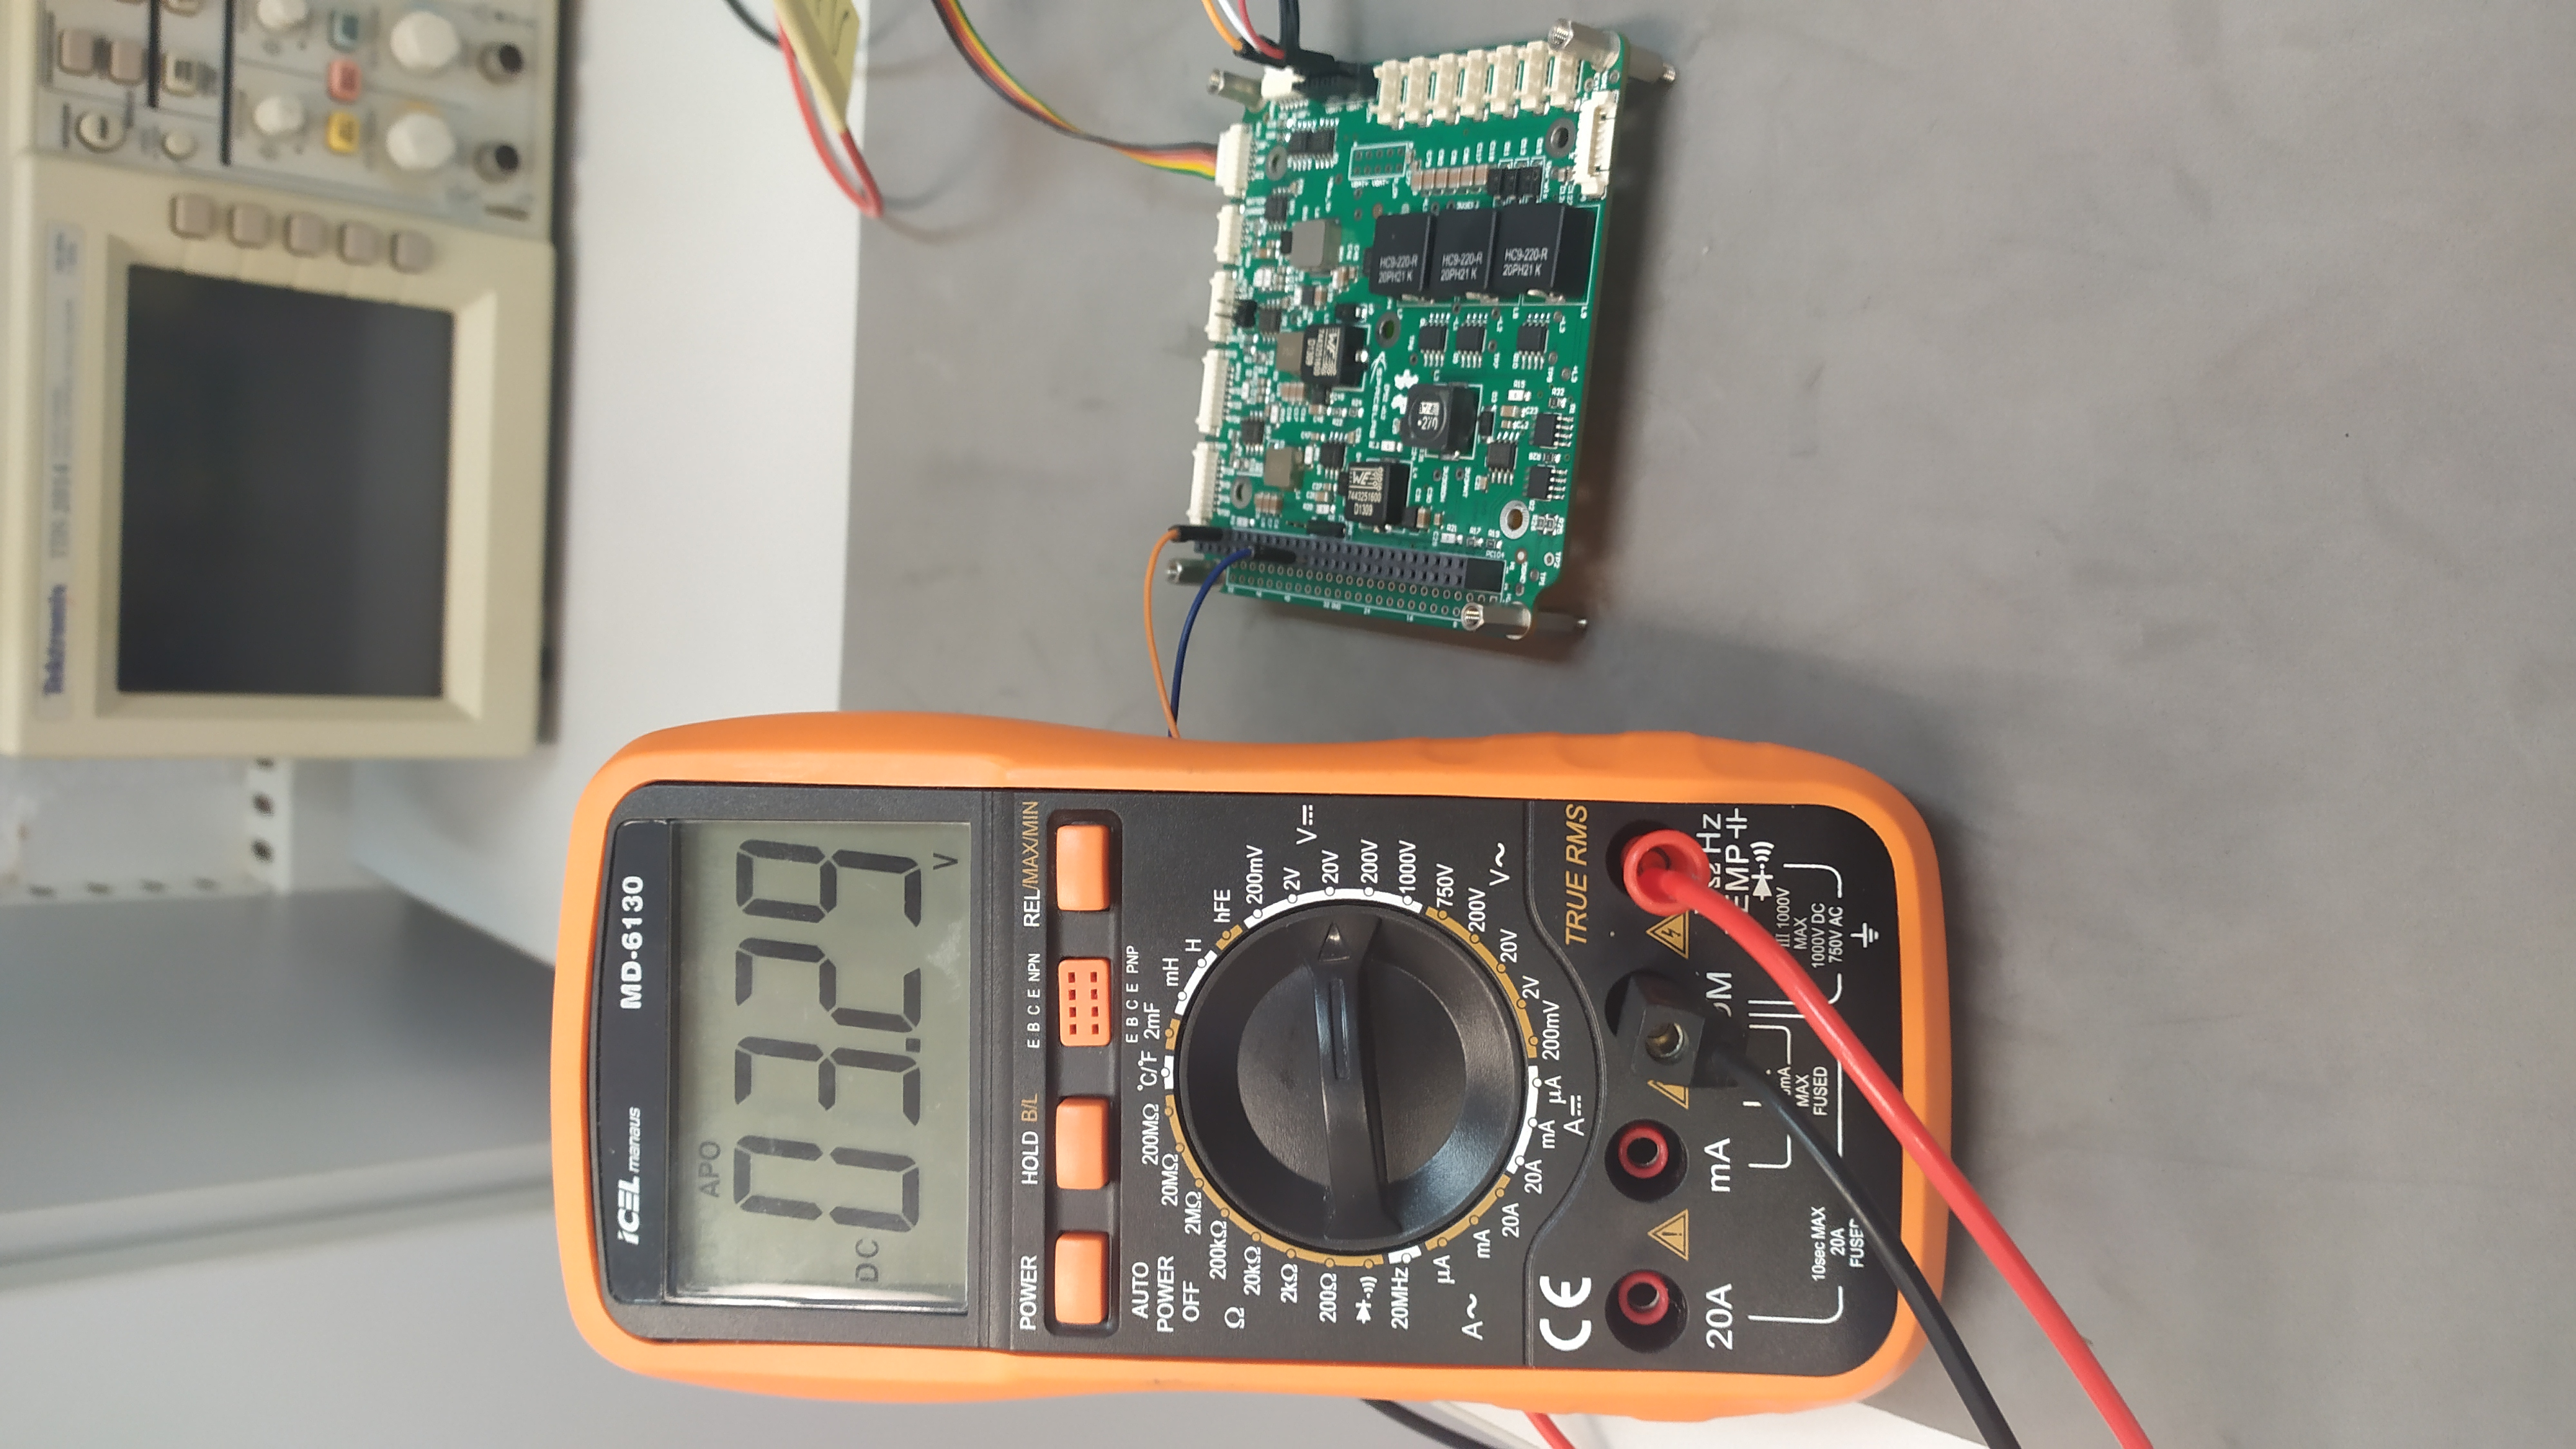
\includegraphics[angle=270,width=0.35\linewidth]{figures/v02/3v3_all_modules_buses.jpg}}        

        \caption{Measuring the voltage of the power buses without a load.}
        \label{fig:regulators_no_load}
    \end{center}
\end{figure}

\begin{itemize}
    \item \textbf{Test description/Objective}: Perform basic tests to evaluate the board with nominal operating parameters.
    \item \textbf{Procedures:} \autoref{tab:electrical-testing}.
    \item \textbf{Material}:
        \begin{itemize}
            \item Fluke's DMMs (Digital Multimeters) from 170 series
            \item N6705B, Keysigh's DC Power Analyser
        \end{itemize}
    \item \textbf{Results}: First, the multimeter was used to search for short circuits between the VCC and GND buses. Then, the EPS 2.0 was turned on with a power supply. Moreover, it was measured the voltage on the power buses without any load, which the results are presented in \autoref{fig:regulators_no_load}. Furthermore, a load was connected to these buses to evaluate if it would occur a voltage drop. The setup for 5V and 6V is shown in \autoref{fig:5v_6v_setup_test} and for 3,3V is shown on \autoref{fig:3v3_setup_test}. For these setups, the load would drain approximately 1A.
    \item \textbf{Conclusion}: The board turned on as expected and present stable power consumption. The voltage at the output of the step-down regulator of the 3,3V bus to power up the Beacon had a significant drop. The issue might be related to poor sizing of passive components required for the regulators. This problem \textbf{must} be solved for the next version (it is expected to be performed minor changes in components values).  
\end{itemize}

\begin{figure}[!ht]
    \begin{center}
        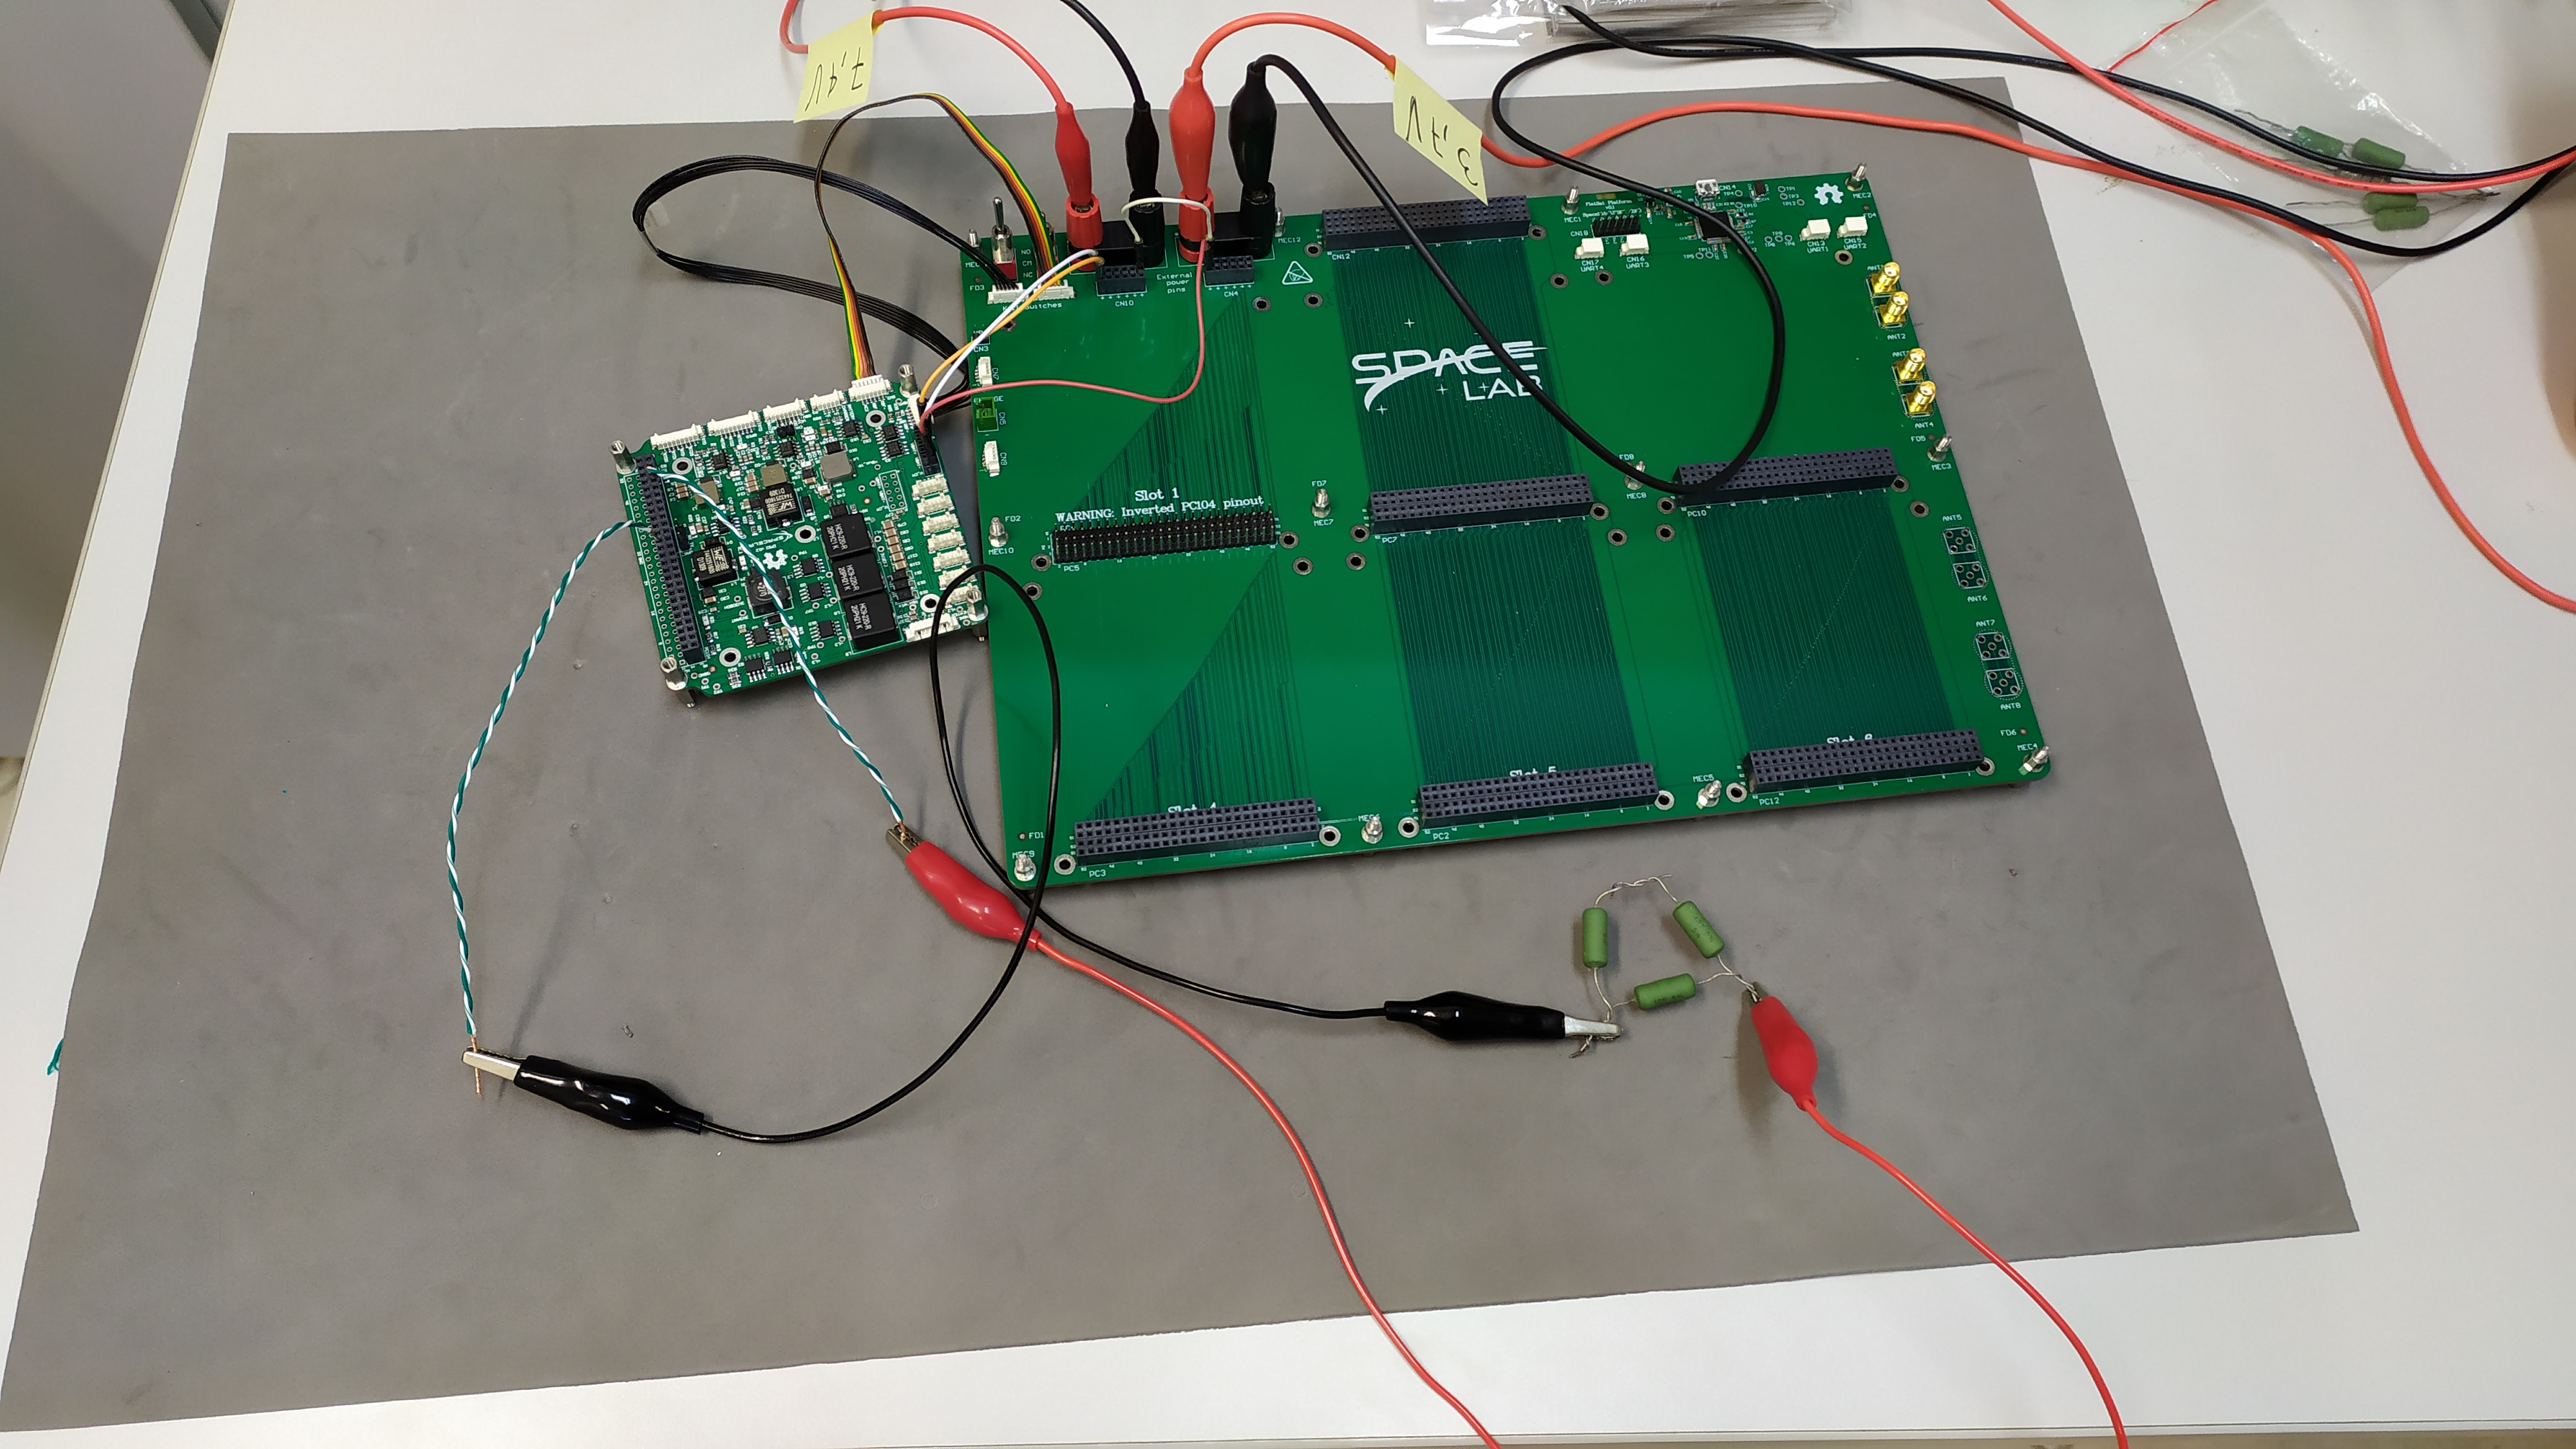
\includegraphics[width=\columnwidth]{figures/v02/5v_6v_setup_test.jpg}
        \caption{Setup to evaluate the 5V and 6V buses with load.}
        \label{fig:5v_6v_setup_test}
    \end{center}
\end{figure}

\newpage

\begin{figure}[!ht]
    \begin{center}
        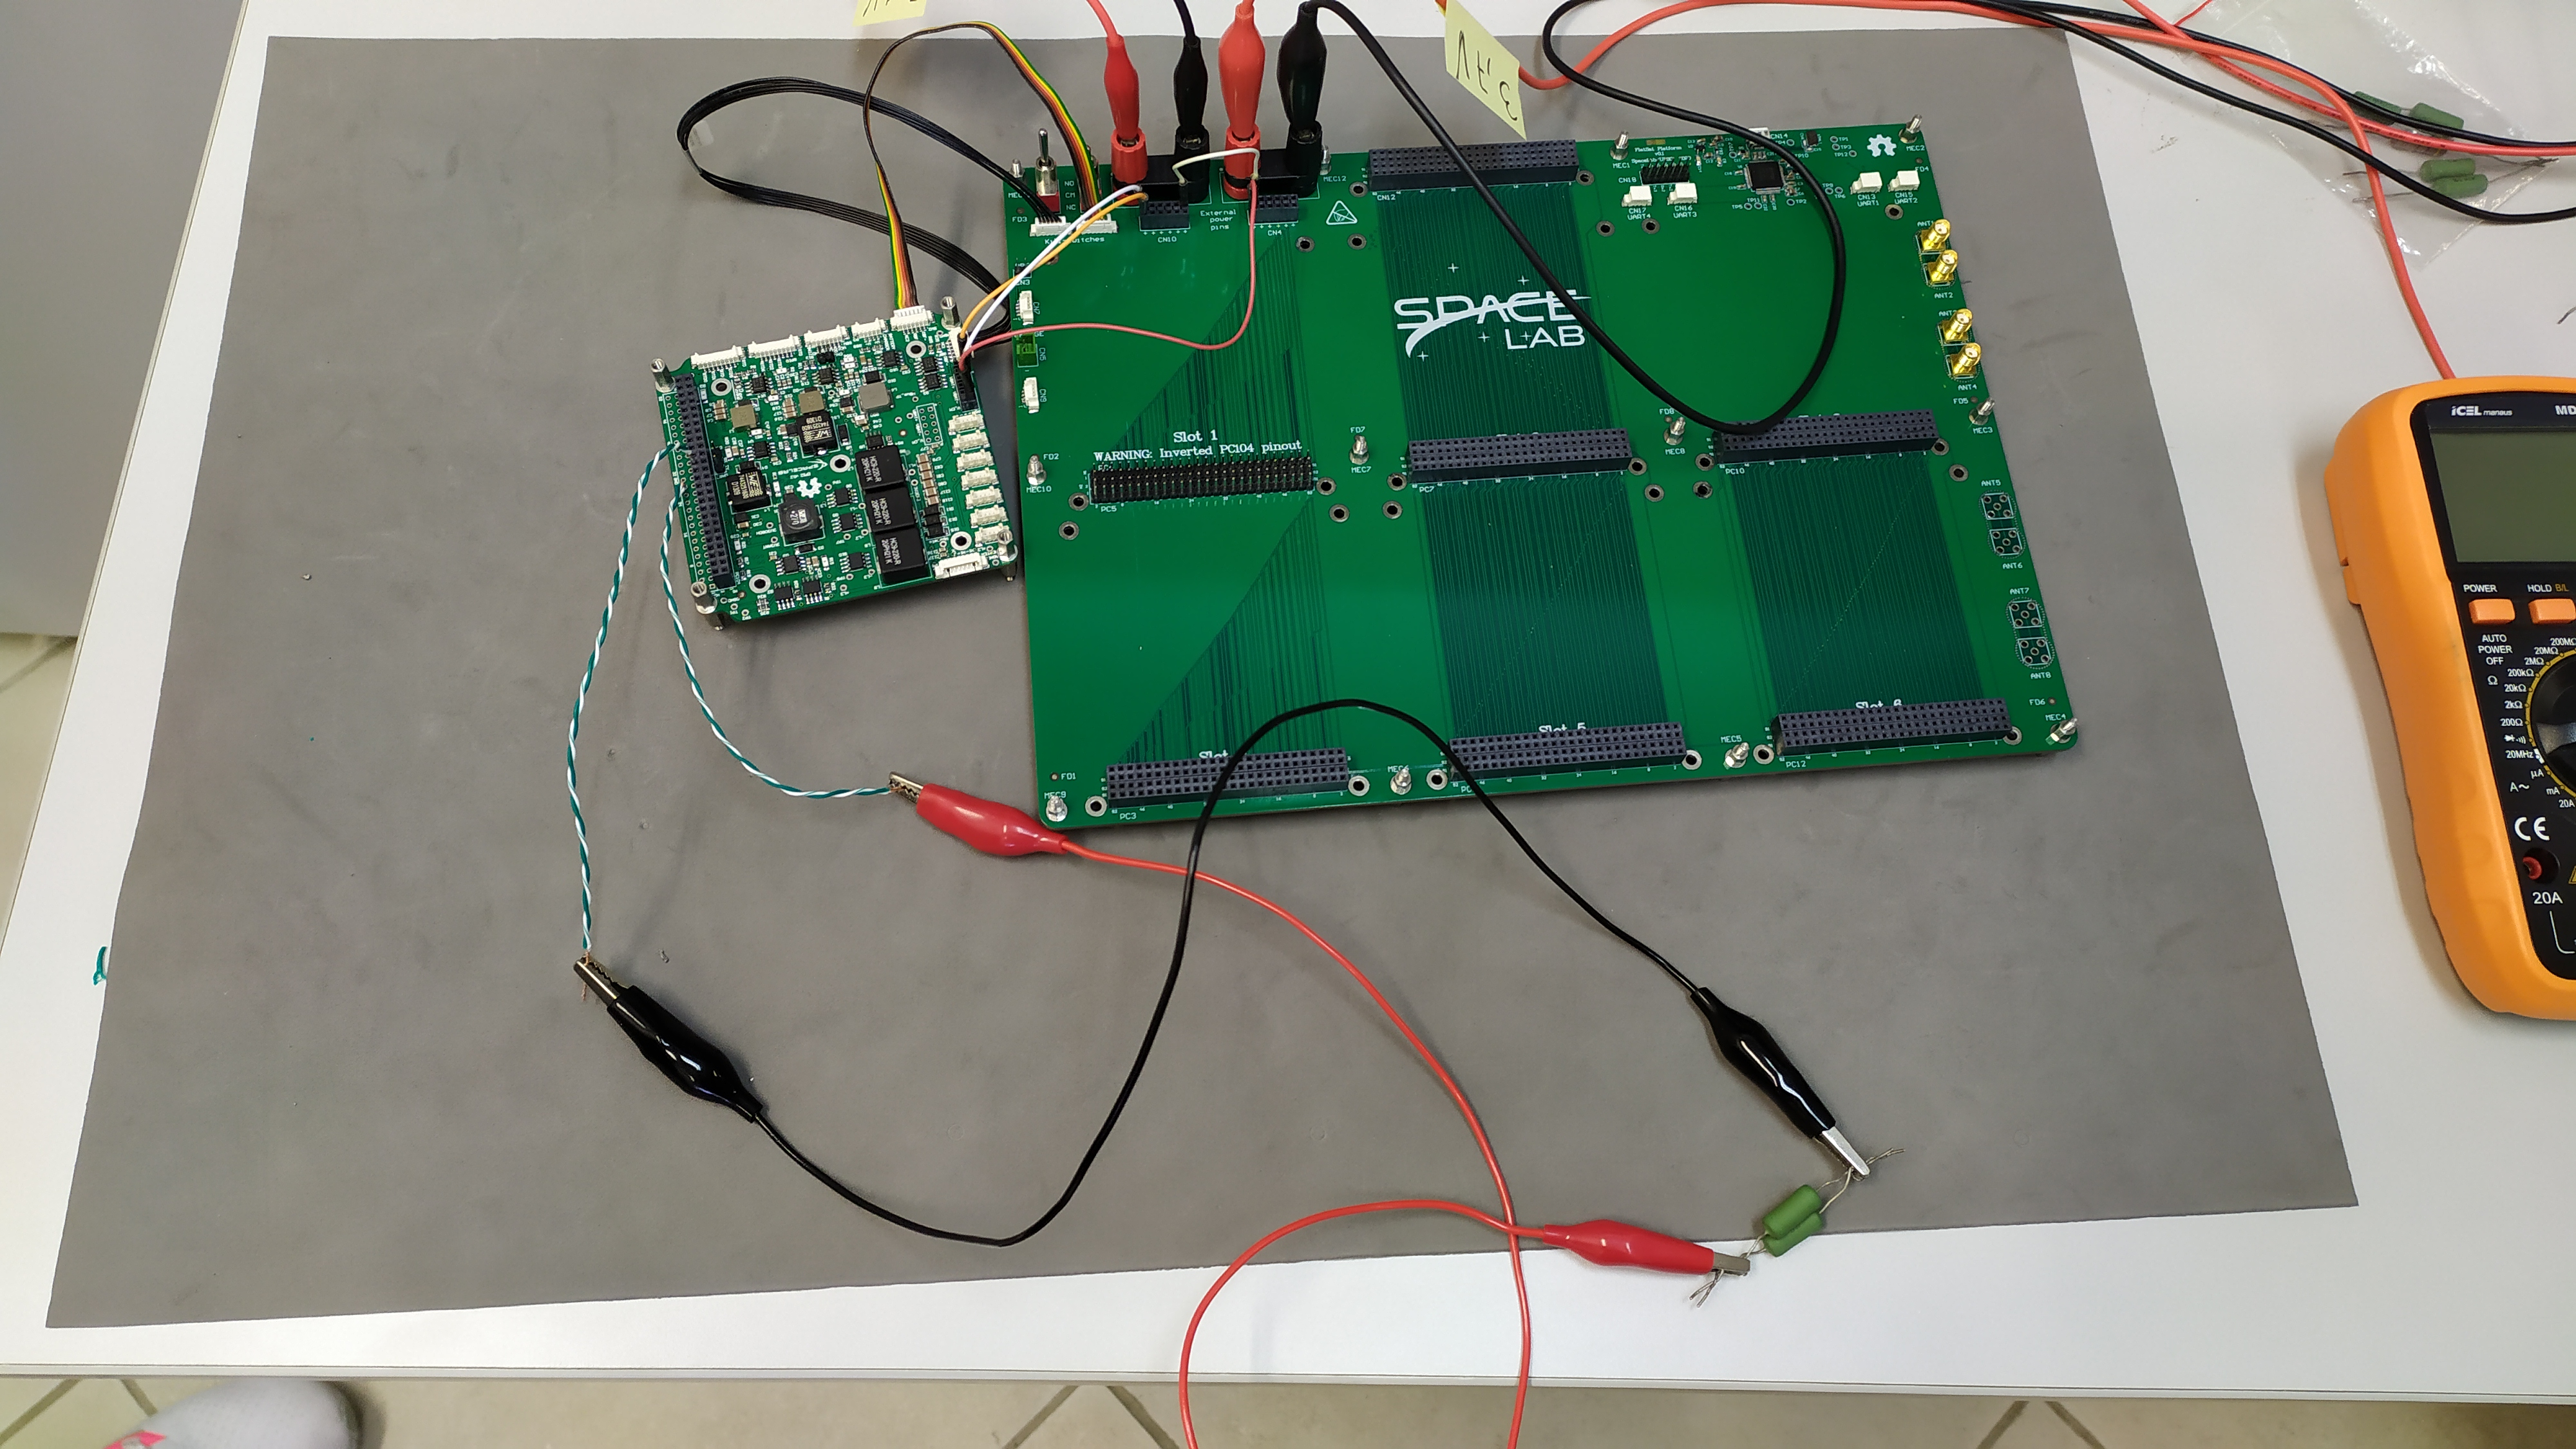
\includegraphics[width=\columnwidth]{figures/v02/3v3_setup_test.jpg}
        \caption{Setup to evaluate the 3,3V buses with load.}
        \label{fig:3v3_setup_test}
    \end{center}
\end{figure}

\section{Functional Testing}

\subsection{Firmware Programming}

\begin{figure}[!htb]
    \begin{center}
        \subfigure[Board connections using the MSP-FET and USB-UART converter.\label{fig:setup-first-boot}]{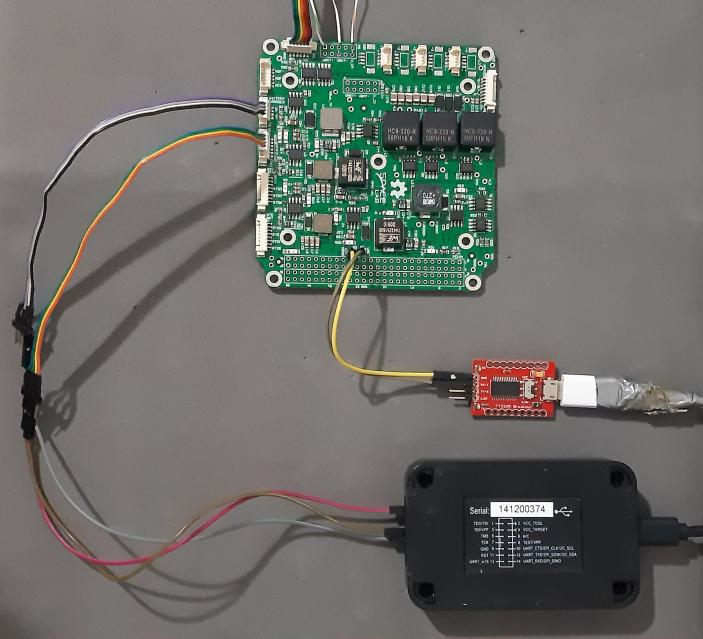
\includegraphics[height=0.23\textheight]{figures/v01/setup-first-boot.jpg}}
        ~
        \subfigure[Pin connections using the MSP-FET and USB-UART converter.\label{fig:electrical-test-board}]{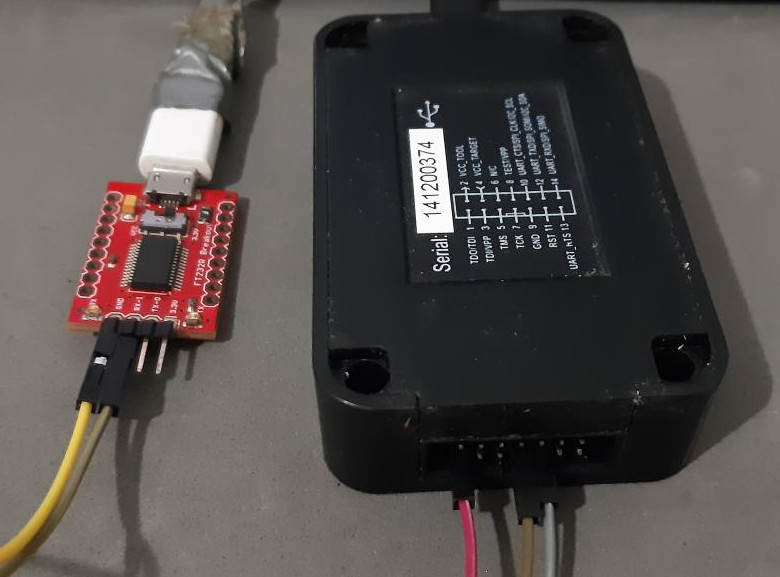
\includegraphics[height=0.23\textheight]{figures/v01/tools-first-boot.jpg}}
        \caption{Setup used for the first firmware boot}
        \label{fig:setup-first-boot}
    \end{center}
\end{figure}

\begin{itemize}
    \item \textbf{Test description/Objective}: Evaluate the board behavior under a firmware programming sequence.
    \item \textbf{Material}:
        \begin{itemize}
            \item Code Composer Studio v10.0.0
            \item MSP-FET Flash Emulation Tool
            \item USB-UART converter
            \item PuTTy
        \end{itemize}
    \item \textbf{Results}: The results of this are available in \autoref{fig:log-first-boot}, where the log messages of the first boot of the board can be seen.
    \item \textbf{Conclusion}: Major problems were identified on this test, but it was expected since the available firmware version was at early stages of refactoring and development.
\end{itemize}

\begin{figure}[!ht]
    \begin{center}
        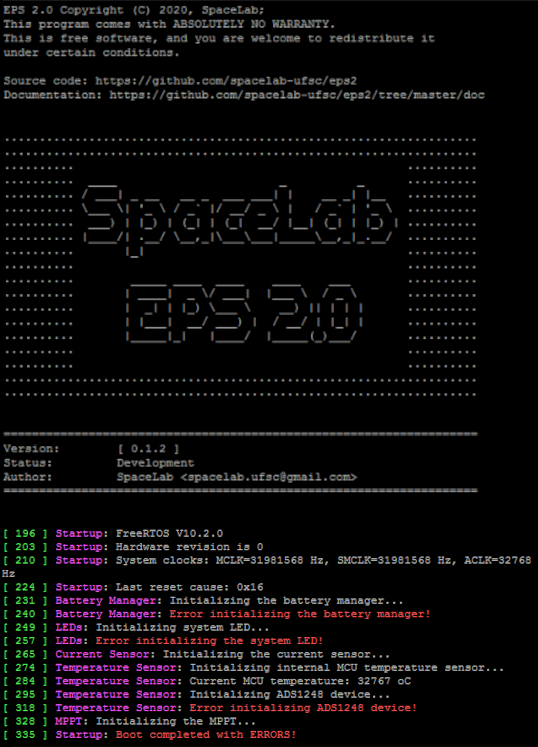
\includegraphics[width=0.6\columnwidth]{figures/v01/log-first-boot.png}
        \caption{Log messages during the first boot.}
        \label{fig:log-first-boot}
    \end{center}
\end{figure}

\subsection{Communication Buses}

\begin{itemize}
    \item \textbf{Test description/Objective}: Test the communication buses of the board, as listed below:
        \begin{itemize}
            \item I$^{2}$C bus, to communicate with the OBDH
            \item UART bus, to communicate with the TTC
        \end{itemize}
    \item \textbf{Material}:
        \begin{itemize}
            \item Saleae Logic Analyzer (24 MHz, 8 channels)
            \item Saleae Logic software (v1.2.18)
            \item MSP-FET Flash Emulation Tool
        \end{itemize}
    \item \textbf{Results}: The results of this test can be seen in \autoref{fig:test-i2c} and \autoref{fig:test-uart}
    \item \textbf{Conclusion:} Minor problems were identified on this test, but were corrected. The figures shows the buses after the corrections, working as expected.
\end{itemize}

\begin{figure}[!htb]
    \begin{center}
        \subfigure[View of the communication.\label{fig:test-uart-1}]{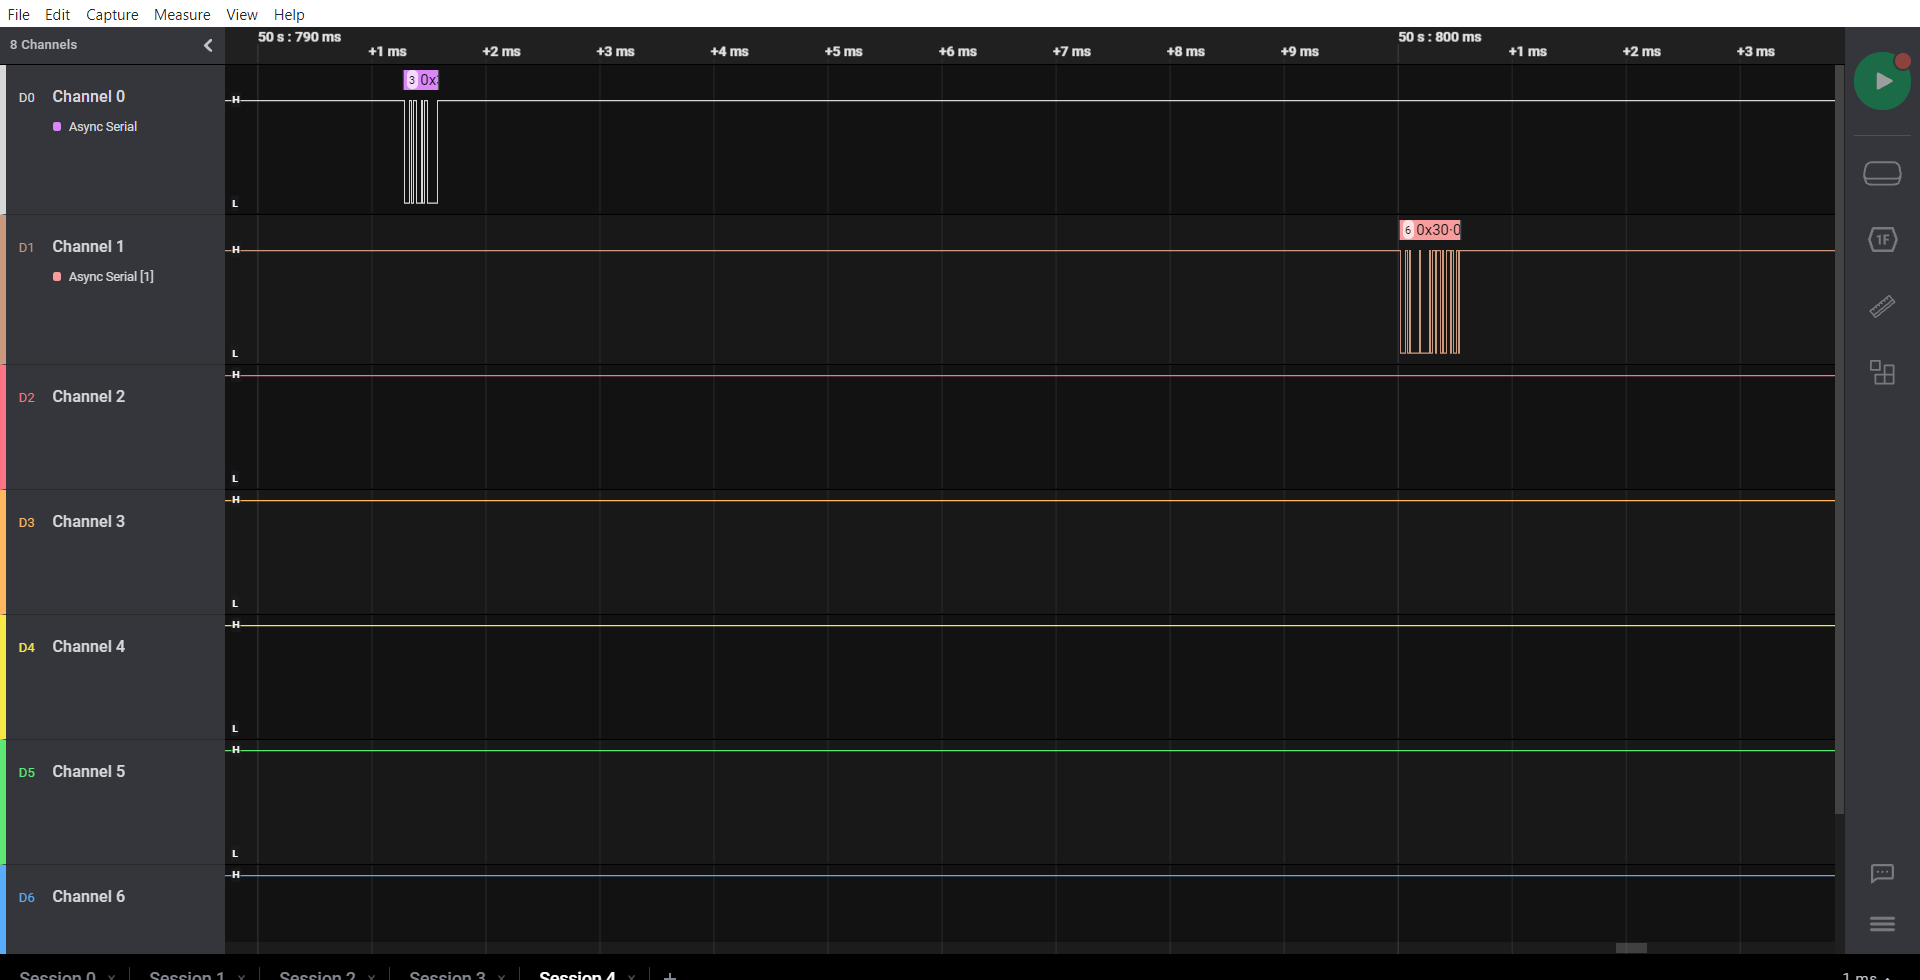
\includegraphics[height=0.25\textheight]{figures/eps_uart_protocol_experiment.png}}
        ~
        \subfigure[Zoom in the data sent by EPS.\label{fig:test-uart-2}]{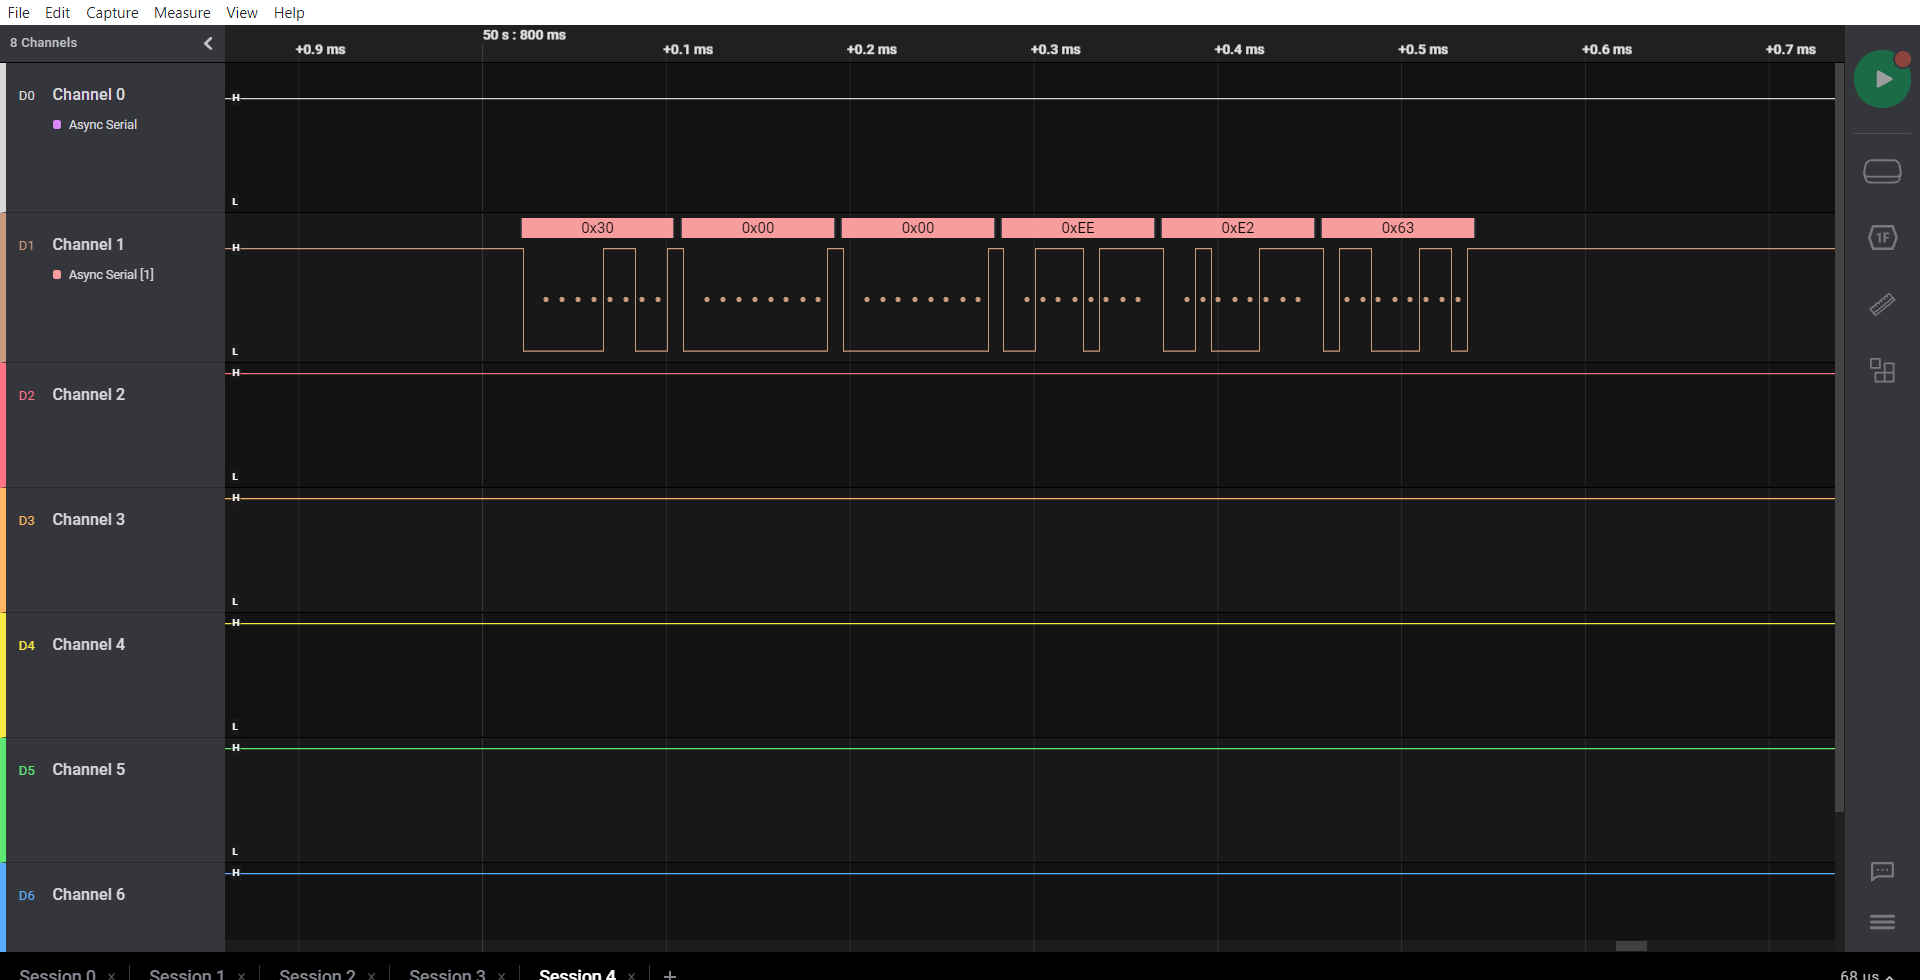
\includegraphics[height=0.25\textheight]{figures/eps_uart_protocol_experiment_zoom.png}}
        \caption{Communication between the TTC and EPS}
        \label{fig:test-uart}
    \end{center}
\end{figure}

\begin{figure}[!ht]
    \begin{center}
        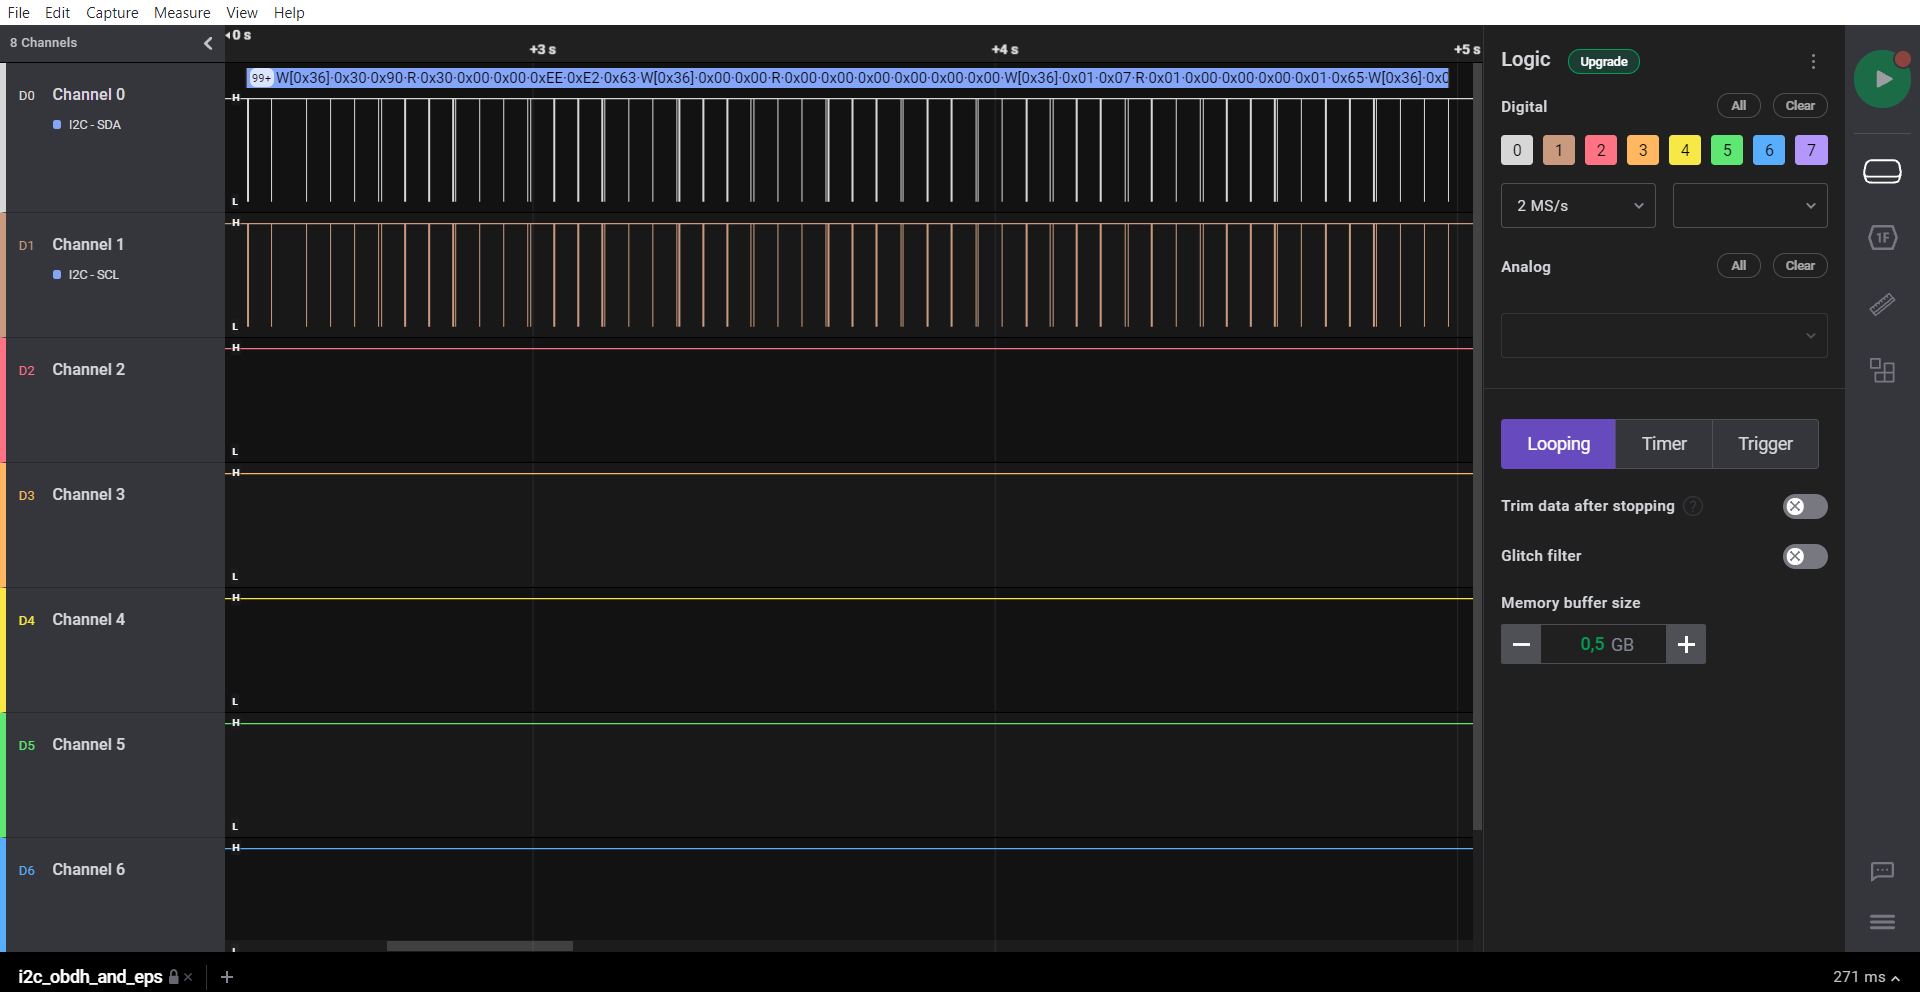
\includegraphics[width=\columnwidth]{figures/eps_i2c_protocol_experiment.png}
        \caption{Communication between the OBDH and EPS.}
        \label{fig:test-i2c}
    \end{center}
\end{figure}

\subsection{Sensors}

\begin{itemize}
    \item \textbf{Test description/Objective}: Test the EPSs' sensors, as listed below:
        \begin{itemize}
            \item Voltage sensors
            \item Current sensors
            \item Temperature sensors
        \end{itemize}
    \item \textbf{Material}:
        \begin{itemize}
            \item Code Composer Studio v9.3.0
            \item MSP-FET Flash Emulation Tool
            \item USB-UART converter
            \item Screen (Linux software)
        \end{itemize}
    \item \textbf{Results}: The values of current, voltage and temperature are correct. The temperature values are shown in \autoref{fig:test-temperature}. The values shown in the figure were obtained during the tests of the heater's on-off controller.
    \item \textbf{Conclusion:} In a first moment, the values of voltage and current were not correct, but it was figured out that the problem was in the firmware. The values of temperature were, in a first moment, all 0$^{\circ}$C. But, again, the problem was in the configuration of the ADS1248. When these problems were corrected, the values started to be correct.
\end{itemize}

\newpage

\begin{figure}[!ht]
    \begin{center}
        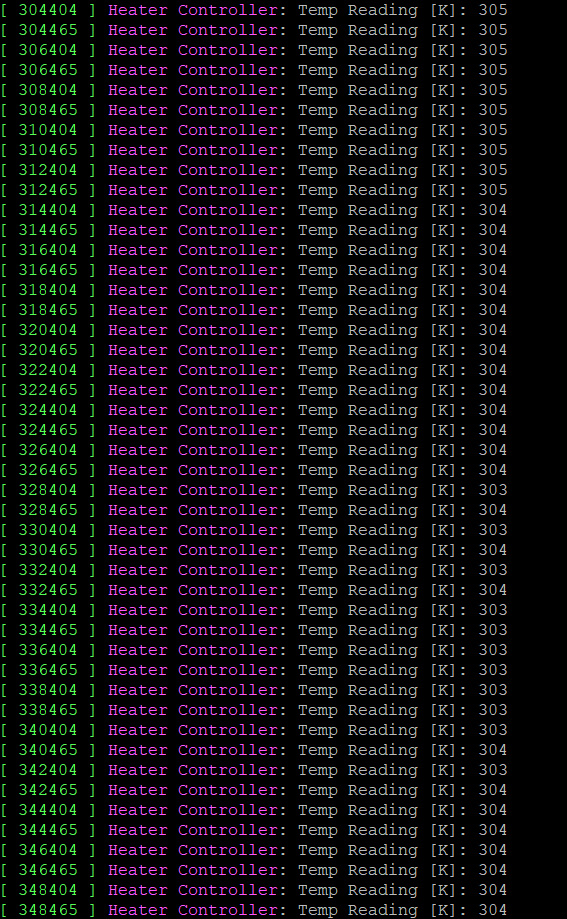
\includegraphics[width=0.5\columnwidth]{figures/test_heater.PNG}
        \caption{Values of temperature during the evaluation of heater's on-off controller.}
        \label{fig:test-temperature}
    \end{center}
\end{figure}

\subsection{Peripherals}

\subsection{Battery monitor}

\begin{itemize}
    \item \textbf{Test description/Objective}: Test the functionality of the DS2777.
    \item \textbf{Material}:
        \begin{itemize}
            \item Saleae Logic Analyzer (24 MHz, 8 channels)
            \item Saleae Logic software (v1.2.18)
            \item MSP-FET Flash Emulation Tool
        \end{itemize}
    \item \textbf{Results}: The results of this test can be seen in \autoref{fig:test-battery-monitor-1}, \autoref{fig:test-battery-monitor-2} and \autoref{fig:test-battery-monitor-3}.
    \item \textbf{Conclusion:} In a first moment, the CI was not working as expected. It was found that the Zener diode, D6, was interfering in the I$^{2}$C communication. It was removed and the CI started to work properly.  
\end{itemize}

\begin{figure}[!ht]
    \begin{center}
        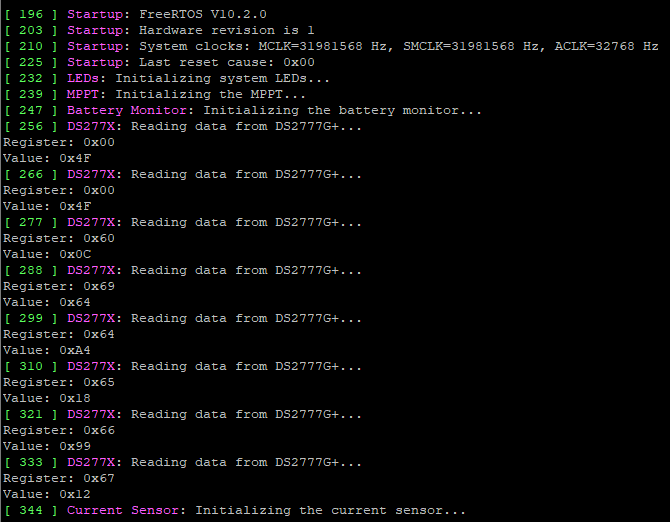
\includegraphics[width=0.7\columnwidth]{figures/ds2777g_log_1.png}
        \caption{First part of the log.}
        \label{fig:test-battery-monitor-1}
    \end{center}
\end{figure}

\begin{figure}[!ht]
    \begin{center}
        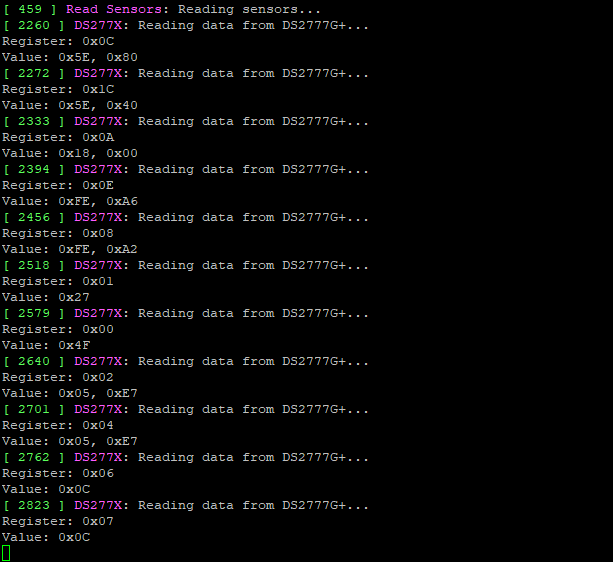
\includegraphics[width=0.7\columnwidth]{figures/ds2777g_log_2.png}
        \caption{Second part of the log.}
        \label{fig:test-battery-monitor-2}
    \end{center}
\end{figure}

\newpage

\begin{figure}[!ht]
    \begin{center}
        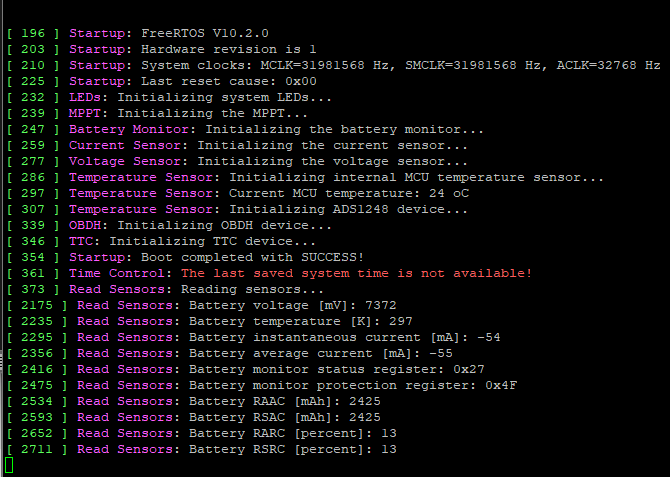
\includegraphics[width=0.7\columnwidth]{figures/ds2777g_log_3.png}
        \caption{Last part of the log.}
        \label{fig:test-battery-monitor-3}
    \end{center}
\end{figure}

\subsection{Heater's on-off controller}

\begin{itemize}
    \item \textbf{Test description/Objective}: Test the functionality of the heater's on-off controller.
    \item \textbf{Material}:
        \begin{itemize}
            \item Logs
            \item MSP-FET Flash Emulation Tool
        \end{itemize}
    \item \textbf{Results}: The results of this test can be seen in \autoref{fig:test-temperature-control}.
    \item \textbf{Conclusion:} The heater's on-off controller is working as expected. It was decided to used, during the tests in the workbench, thresholds such 26$^{\circ}$C and 32$^{\circ}$C.  
\end{itemize}

\begin{figure}[!ht]
    \begin{center}
        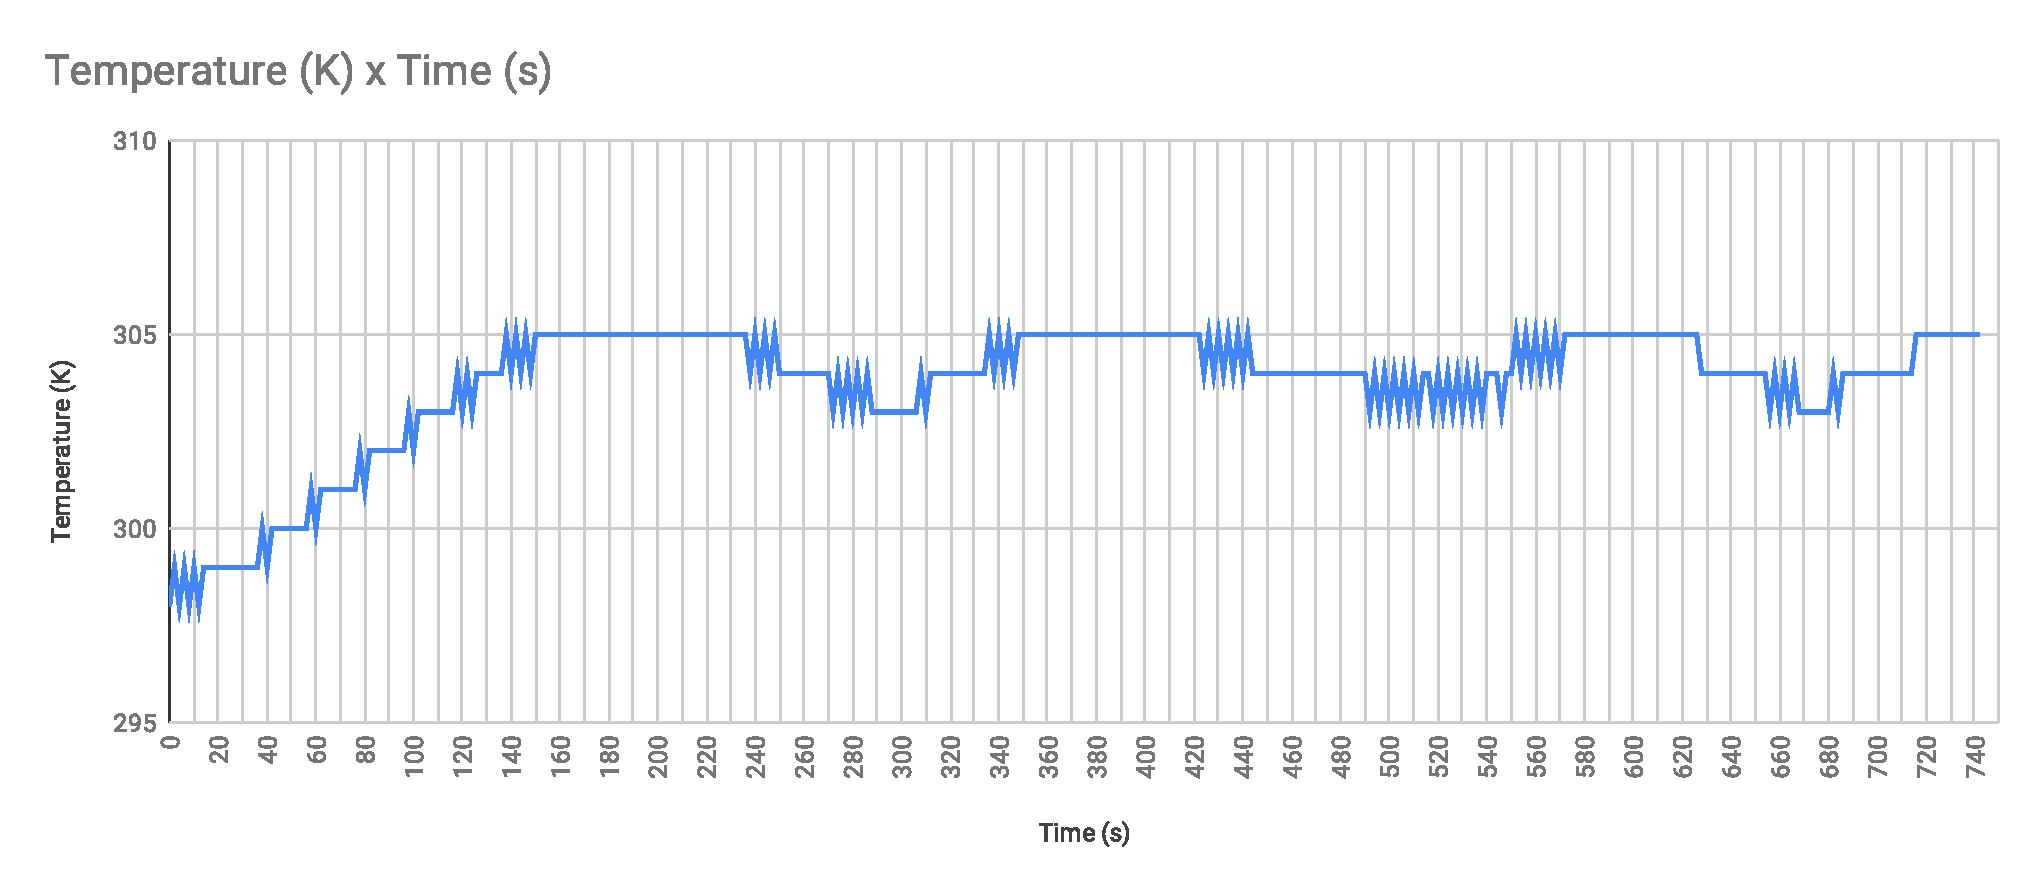
\includegraphics[width=\columnwidth]{figures/heater_controller.pdf}
        \caption{Temperature of the batteries being controlled.}
        \label{fig:test-temperature-control}
    \end{center}
\end{figure}

\subsection{MPPT controller}

\begin{itemize}
    \item \textbf{Test description/Objective}: Test the functionality of the MPPT controller.
    \item \textbf{Material}:
        \begin{itemize}
            \item Oscilloscope
            \item Unit tests
            \item MSP-FET Flash Emulation Tool
        \end{itemize}
    \item \textbf{Results}: The PWM signal generated by the MPPT controller can be seen in \autoref{fig:test-pwm-1} and \autoref{fig:test-pwm-2}, as well as the test workflow can be accessed in the GitHub page.
    \item \textbf{Conclusion:} The algorithm was tested using the unit tests, and worked as expected. The PWM signal for 100kHz and 50kHz are being generated correctly.  
\end{itemize}

\begin{figure}[!ht]
    \begin{center}
        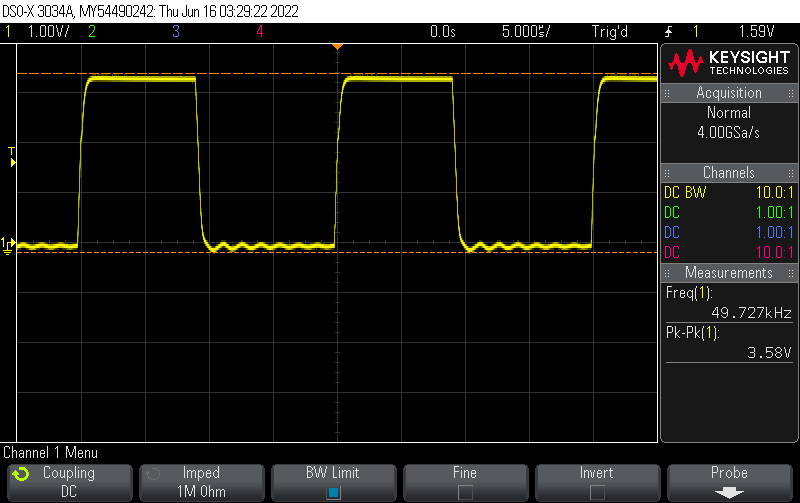
\includegraphics[width=0.6\columnwidth]{figures/eps_pwm_50khz.png}
        \caption{PWM signal, at 50kHz, generated by the MPPT controller.}
        \label{fig:test-pwm-1}
    \end{center}
\end{figure}

\begin{figure}[!ht]
    \begin{center}
        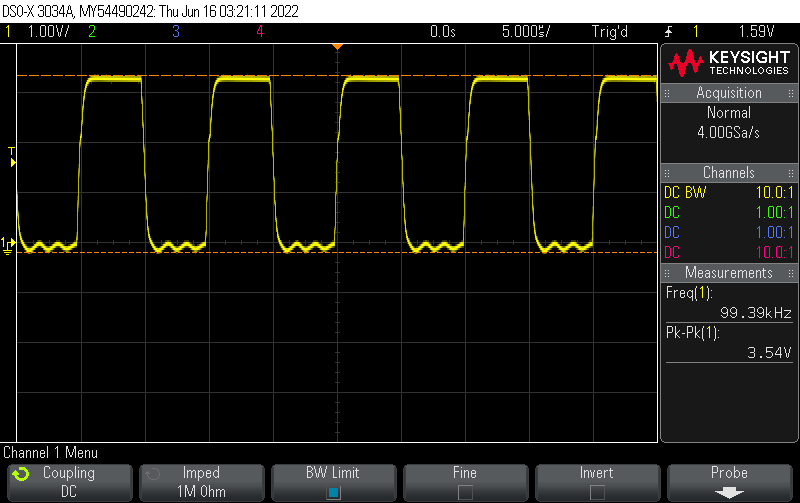
\includegraphics[width=0.6\columnwidth]{figures/eps_pwm_100khz.png}
        \caption{PWM signal, at 100kHz, generated by the MPPT controller.}
        \label{fig:test-pwm-2}
    \end{center}
\end{figure}

\section{Conclusion} The board can be connected with the rest of the satellite, using a FlatSat platform, to make system level tests.
